\documentclass[aps,prb,reprint,noshowkeys,linenumbers,superscriptaddress]{revtex4-1}
\usepackage{subcaption}
\usepackage{bm,graphicx,tabularx,array,booktabs,dcolumn,xcolor,microtype,multirow,amscd,amsmath,amssymb,amsfonts,physics,siunitx,mhchem}
\usepackage[utf8]{inputenc}
\usepackage[T1]{fontenc}
\usepackage{txfonts}

\usepackage[normalem]{ulem}
\definecolor{hughgreen}{RGB}{0, 128, 0}
\newcommand{\titou}[1]{\textcolor{red}{#1}}
\newcommand{\hugh}[1]{\textcolor{hughgreen}{#1}}
\newcommand{\trash}[1]{\textcolor{red}{\sout{#1}}}
\newcommand{\trashHB}[1]{\textcolor{orange}{\sout{#1}}}

\usepackage[
	colorlinks=true,
    citecolor=blue,
    linkcolor=blue,
    filecolor=blue,      
    urlcolor=blue,	
    breaklinks=true
	]{hyperref}
\urlstyle{same}

\newcommand{\ctab}{\multicolumn{1}{c}{---}}
\newcommand{\latin}[1]{#1}
%\newcommand{\latin}[1]{\textit{#1}}
\newcommand{\ie}{\latin{i.e.}}
\newcommand{\eg}{\latin{e.g.}}
\newcommand{\etal}{\textit{et al.}}

\newcommand{\mc}{\multicolumn}
\newcommand{\fnm}{\footnotemark}
\newcommand{\fnt}{\footnotetext}
\newcommand{\mcc}[1]{\multicolumn{1}{c}{#1}}
\newcommand{\mr}{\multirow}

% operators
\newcommand{\bH}{\mathbf{H}}
\newcommand{\bV}{\mathbf{V}}
\newcommand{\bh}{\mathbf{h}}
\newcommand{\bQ}{\mathbf{Q}}
\newcommand{\bSig}{\mathbf{\Sigma}}
\newcommand{\br}{\mathbf{r}}
\newcommand{\bp}{\mathbf{p}}
\newcommand{\cP}{\mathcal{P}}
\newcommand{\cS}{\mathcal{S}}
\newcommand{\cT}{\mathcal{T}}
\newcommand{\cC}{\mathcal{C}}
\newcommand{\PT}{\mathcal{PT}}

\newcommand{\EPT}{E_{\PT}}
\newcommand{\laPT}{\lambda_{\PT}}

\newcommand{\EEP}{E_\text{EP}}
\newcommand{\laEP}{\lambda_\text{EP}}


\newcommand{\Ne}{N} % Number of electrons
\newcommand{\Nn}{M} % Number of nuclei
\newcommand{\hI}{\Hat{I}}
\newcommand{\hH}{\Hat{H}}
\newcommand{\hS}{\Hat{S}}
\newcommand{\hT}{\Hat{T}}
\newcommand{\hW}{\Hat{W}}
\newcommand{\hV}{\Hat{V}}
\newcommand{\hc}[2]{\Hat{c}_{#1}^{#2}}
\newcommand{\hn}[1]{\Hat{n}_{#1}}
\newcommand{\n}[1]{n_{#1}}
\newcommand{\Dv}{\Delta v}

\newcommand{\ra}{\rightarrow}
\newcommand{\up}{\uparrow}
\newcommand{\dw}{\downarrow}

\newcommand{\updot}{%
  \mathrel{\ooalign{\hfil$\vcenter{
    \hbox{$\scriptscriptstyle\bullet$}}$\hfil\cr$\uparrow$\cr}
  }%
}
\newcommand{\dwdot}{%
  \mathrel{\ooalign{\hfil$\vcenter{
    \hbox{$\scriptscriptstyle\bullet$}}$\hfil\cr$\downarrow$\cr}
  }%
}
\newcommand{\vac}{%
  \mathrel{\ooalign{\hfil$\vcenter{
    \hbox{$\scriptscriptstyle\bullet$}}$\hfil\cr$ $\cr}
  }%
}

\newcommand{\uddot}{%
  \mathrel{\ooalign{\hfil$\vcenter{
    \hbox{$\scriptscriptstyle\bullet$}}$\hfil\cr$\uparrow\downarrow$\cr}
  }%
}

% Center tabularx columns
\newcolumntype{Y}{>{\centering\arraybackslash}X}

% HF rotation angles
\newcommand{\ta}{\theta_{\alpha}}
\newcommand{\tb}{\theta_{\beta}}

% Some constants
\renewcommand{\i}{\mathrm{i}} % Imaginary unit
\newcommand{\e}{\mathrm{e}} % Euler number
\newcommand{\rc}{r_{\text{c}}}
\newcommand{\lc}{\lambda_{\text{c}}}
\newcommand{\lep}{\lambda_{\text{EP}}}

% Some energies
\newcommand{\Emp}{E_{\text{MP}}}

% Blackboard bold
\newcommand{\bbR}{\mathbb{R}}
\newcommand{\bbC}{\mathbb{C}}

\newcommand{\Lup}{\mathcal{L}^{\uparrow}}
\newcommand{\Ldown}{\mathcal{L}^{\downarrow}}
\newcommand{\Lsi}{\mathcal{L}^{\sigma}}
\newcommand{\Rup}{\mathcal{R}^{\uparrow}}
\newcommand{\Rdown}{\mathcal{R}^{\downarrow}}
\newcommand{\Rsi}{\mathcal{R}^{\sigma}}


\newcommand{\LCPQ}{Laboratoire de Chimie et Physique Quantiques (UMR 5626), Universit\'e de Toulouse, CNRS, UPS, France.}
\newcommand{\UCAM}{Department of Chemistry, University of Cambridge, Lensfield Road, Cambridge, CB2 1EW, U.K.}
\newcommand{\UOX}{Physical and Theoretical Chemical Laboratory, Department of Chemistry, University of Oxford, Oxford, OX1 3QZ, U.K.}
\begin{document}	

\title{Perturbation Theory in the Complex Plane: Exceptional Points and Where to Find Them}

\author{Antoine \surname{Marie}}
\affiliation{\LCPQ}
\author{Hugh G.~A.~\surname{Burton}}
\email{hugh.burton@chem.ox.ac.uk}
\affiliation{\UOX}
\author{Pierre-Fran\c{c}ois \surname{Loos}}
\email{loos@irsamc.ups-tlse.fr}
\affiliation{\LCPQ}


\begin{abstract}
In this review, we explore the extension of quantum chemistry in the complex plane and its link with perturbation theory.
We observe that the physics of a quantum system is intimately connected to the position of energy singularities in the complex plane, known as exceptionnal points.
After a presentation of the fundamental notions of quantum chemistry in the complex plane, such as the mean-field Hartree-Fock approximation and Rayleigh-Schr\"odinger perturbation theory, and their illustration with the ubiquitous (symmetric) Hubbard dimer at half filling, we provide a historical overview of the various research activities that have been performed on the physics of singularities.
In particular, we highlight the seminal work of several research groups on the convergence behaviour of perturbative series obtained within M{\o}ller--Plesset perturbation theory and its apparent link with quantum phase transitions.
\end{abstract}

\maketitle

\raggedbottom
\tableofcontents

%%%%%%%%%%%%%%%%%%%%%%%
\section{Introduction}
\label{sec:intro}
%%%%%%%%%%%%%%%%%%%%%%%

Due to the ubiquitous influence of processes involving electronic states in physics, chemistry, and biology, their faithful description from first principles has been one of the grand challenges faced by theoretical chemists since the dawn of computational chemistry. 
Accurately predicting ground- and excited-state energies (hence excitation energies) is particularly valuable in this context, and it has concentrated most of the efforts within the community.
An armada of theoretical and computational methods have been developed to this end, each of them being plagued by its own flaws. 
The fact that none of these methods is successful in every chemical scenario has encouraged chemists to carry on the development of new methodologies, their main goal being to get the most accurate energies (and properties) at the lowest possible computational cost in the most general context.

One common feature of all these methods is that they rely on the notion of quantised energy levels of Hermitian quantum mechanics, in which the different electronic states of a molecule or an atom are energetically ordered, the lowest being the ground state while the higher ones are excited states. 
Within this quantised paradigm, electronic states look completely disconnected from one another.
Many current methods study excited states using only ground-state information, creating a ground-state bias that leads to incorrect excitation energies.
However, one can gain a different perspective on quantisation extending quantum chemistry into the complex domain.
In a non-Hermitian complex picture, the energy levels are \textit{sheets} of a more complicated topological manifold called \textit{Riemann surface}, and they are smooth and continuous \textit{analytic continuation} of one another. 
In other words, our view of the quantised nature of conventional Hermitian quantum mechanics arises only from our limited perception of the more complex and profound structure of its non-Hermitian variant. \cite{MoiseyevBook,BenderPTBook}
The realisation that ground and excited states both emerge from one single mathematical structure with equal importance suggests that excited-state energies can be computed from first principles in their own right. 
One could then exploit the structure of these Riemann surfaces to develop methods that directly target excited-state energies without needing ground-state information. \cite{Burton_2019,Burton_2019a}

By analytically continuing the electronic energy $E(\lambda)$ in the complex domain (where $\lambda$ is a coupling parameter), the ground and excited states of a molecule can be smoothly connected.
This connection is possible because by extending real numbers to the complex domain, the ordering property of real numbers is lost.
Hence, electronic states can be interchanged away from the real axis since the concept of ground and excited states has been lost.
Amazingly, this smooth and continuous transition from one state to another has recently been experimentally realised in physical settings such as electronics, microwaves, mechanics, acoustics, atomic systems and optics. \cite{Bittner_2012,Chong_2011,Chtchelkatchev_2012,Doppler_2016,Guo_2009,Hang_2013,Liertzer_2012,Longhi_2010,Peng_2014, Peng_2014a,Regensburger_2012,Ruter_2010,Schindler_2011,Szameit_2011,Zhao_2010,Zheng_2013,Choi_2018,El-Ganainy_2018}

Exceptional points (EPs) are branch point singularities where two (or more) states become exactly degenerate. \cite{MoiseyevBook,Heiss_1988,Heiss_1990,Heiss_1999,Berry_2011,Heiss_2012,Heiss_2016,Benda_2018}
They are the non-Hermitian analogs of conical intersections, \cite{Yarkony_1996} which are ubiquitous in non-adiabatic processes and play a key role in photochemical mechanisms.
In the case of auto-ionising resonances, EPs have a role in deactivation processes similar to conical intersections in the decay of bound excited states. \cite{Benda_2018}
Although Hermitian and non-Hermitian Hamiltonians are closely related, the behaviour of their eigenvalues near degeneracies is starkly different.
For example, encircling non-Hermitian degeneracies at EPs leads to an interconversion of states, and two loops around the EP are necessary to recover the initial energy. \cite{MoiseyevBook,Heiss_2016,Benda_2018}
Additionally, the wave function picks up a geometric phase (also known as Berry phase \cite{Berry_1984}) and four loops are required to recover the initial wave function.
In contrast, encircling Hermitian degeneracies at conical intersections only introduces a geometric phase while leaving the states unchanged.
More dramatically, whilst eigenvectors remain orthogonal at conical intersections, at non-Hermitian EPs the eigenvectors themselves become equivalent, resulting in a \textit{self-orthogonal} state. \cite{MoiseyevBook}
More importantly here, although EPs usually lie off the real axis, these singular points are intimately related to the convergence properties of perturbative methods and avoided crossing on the real axis are indicative of singularities in the complex plane. \cite{BenderBook,Olsen_1996,Olsen_2000,Olsen_2019,Mihalka_2017a,Mihalka_2017b,Mihalka_2019}

\titou{The use of non-Hermitian Hamiltonians in quantum chemistry has a long history; these Hamiltonians have been used extensively as a method for describing metastable resonance phenomena. \cite{MoiseyevBook}
Through a complex-scaling of the electronic or atomic coordinates,\cite{Moiseyev_1998} or by introducing a complex absorbing potential,\cite{Riss_1993,Ernzerhof_2006,Benda_2018} outgoing resonance states are transformed into square-integrable wave functions that allow the energy and lifetime of the resonance to be computed.
We refer the interested reader to the excellent book of Moiseyev for a general overview. \cite{MoiseyevBook}}

%%%%%%%%%%%%%%%%%%%%%%%
\section{Exceptional Points in Electronic Structure}
\label{sec:EPs}
%%%%%%%%%%%%%%%%%%%%%%%

%%%%%%%%%%%%%%%%%%%%%%%
\subsection{Time-Independent Schr\"odinger Equation}
\label{sec:TDSE}
%%%%%%%%%%%%%%%%%%%%%%%
Within the Born-Oppenheimer approximation, the exact molecular Hamiltonian with $\Ne$ electrons and 
$\Nn$ (clamped) nuclei is defined for a given nuclear framework as
\begin{equation}\label{eq:ExactHamiltonian}
    \hH(\vb{R}) = 
    - \frac{1}{2} \sum_{i}^{\Ne} \grad_i^2 
    - \sum_{i}^{\Ne} \sum_{A}^{\Nn} \frac{Z_A}{\abs{\vb{r}_i-\vb{R}_A}} 
    + \sum_{i<j}^{\Ne}\frac{1}{\abs{\vb{r}_i-\vb{r}_j}},
\end{equation}
where $\vb{r}_i$ defines the position of the $i$-th electron, $\vb{R}_{A}$ and $Z_{A}$ are the position
and charge of the $A$-th nucleus respectively, and $\vb{R} = (\vb{R}_{1}, \dots, \vb{R}_{\Nn})$ is a
collective vector for the nuclear positions.
The first term represents the kinetic energy of the electrons, while 
the two following terms account for the electron-nucleus attraction and the electron-electron repulsion.

% EXACT SCHRODINGER EQUATION
The exact many-electron wave function at a given nuclear geometry $\Psi(\vb{R})$ corresponds 
to the solution of the (time-independent) Schr\"{o}dinger equation
\begin{equation} 
    \hH(\vb{R})\, \Psi(\vb{R}) = E(\vb{R})\, \Psi(\vb{R}),
    \label{eq:SchrEq}
\end{equation} 
with the eigenvalues $E(\vb{R})$ providing the exact energies.
The energy $E(\vb{R})$ can be considered as a ``one-to-many'' function since each input nuclear geometry
yields several eigenvalues corresponding to the ground and excited states of the exact spectrum.
However, exact solutions to Eq.~\eqref{eq:SchrEq} are only possible in the simplest of systems, such as 
the one-electron hydrogen atom and some specific two-electron systems with well-defined mathematical 
properties.\cite{Taut_1993,Loos_2009b,Loos_2010e,Loos_2012}
In practice, approximations to the exact Schr\"{o}dinger equation must be introduced, including
the perturbation theories and Hartree--Fock approximation considered in this review
In what follows, we will drop the parametric dependence on the nuclear geometry and, 
unless otherwise stated, atomic units will be used throughout.

%===================================%
\subsection{Exceptional Points in the Hubbard Dimer}
\label{sec:example}
%===================================%

%%% FIG 1 %%%
\begin{figure*}[t]
	\begin{subfigure}{0.49\textwidth}
	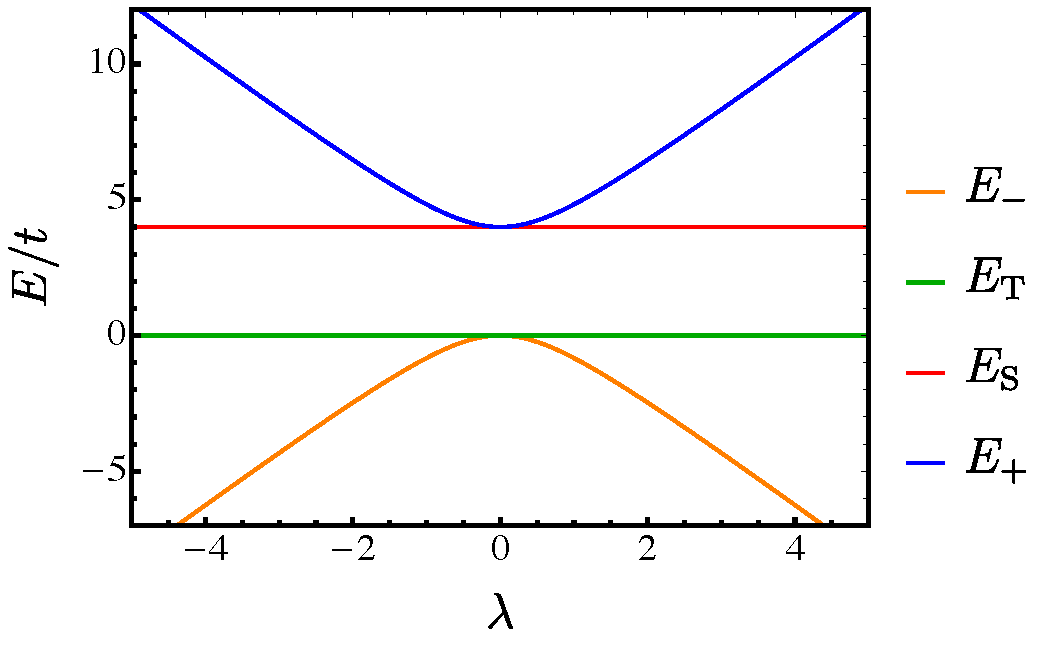
\includegraphics[height=0.65\textwidth]{fig1a}
	\subcaption{\label{subfig:FCI_real}}
    \end{subfigure}
	\begin{subfigure}{0.49\textwidth}
	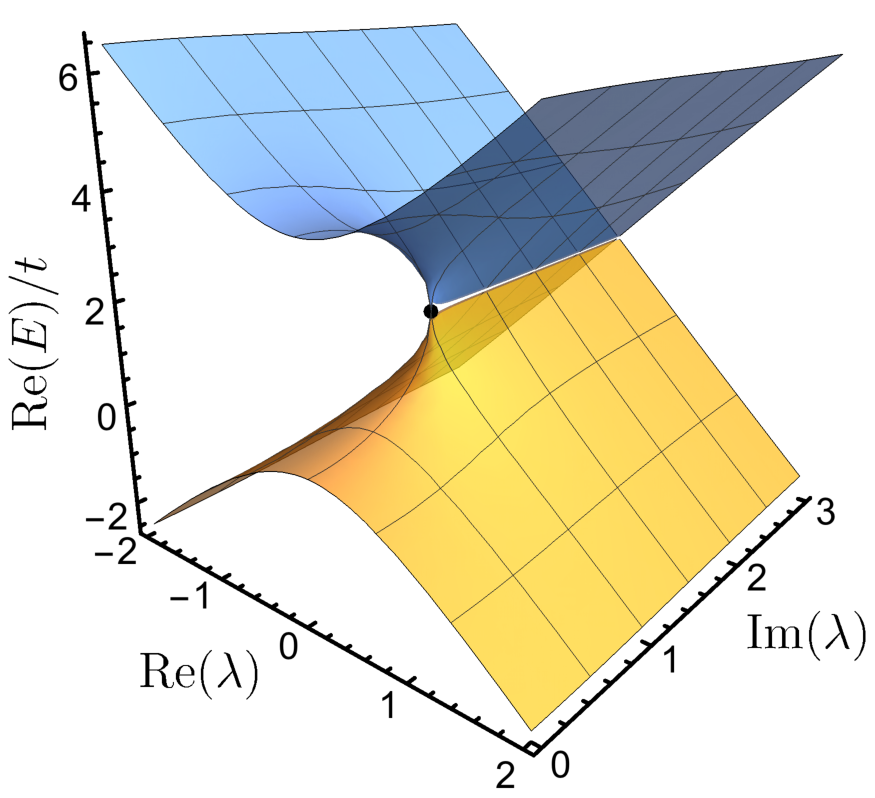
\includegraphics[height=0.65\textwidth]{fig1b}
	\subcaption{\label{subfig:FCI_cplx}}
    \end{subfigure}
	\caption{%
	Exact energies for the Hubbard dimer ($U=4t$) as functions of $\lambda$ on the real axis (\subref{subfig:FCI_real}) and in the complex plane (\subref{subfig:FCI_cplx}).
    Only the interacting closed-shell singlets are plotted in the complex plane, becoming degenerate at the EP (black dot).
    The contour followed around the EP in order to interchange states is also represented.
	\label{fig:FCI}}
\end{figure*}

To illustrate the concepts discussed throughout this article, we consider the symmetric Hubbard dimer at half filling, \ie\ with two opposite-spin fermions.
Analytically solvable models are essential in theoretical chemistry and physics as their mathematical simplicity compared to realistic systems (e.g., atoms and molecules) allows new concepts and methods to be 
easily tested while retaining the key physical phenomena.

Using the (localised) site basis, the Hilbert space of the Hubbard dimer comprises the four configurations
\begin{align*}
& \ket{\Lup \Ldown} &  & \ket{\Lup\Rdown} &  & \ket{\Rup\Ldown} &  & \ket{\Rup\Rdown}
\end{align*}
where $\Lsi$ ($\Rsi$) denotes an electron with spin $\sigma$ on the left (right) site.
The exact, or full configuration interaction (FCI), Hamiltonian is then 
\begin{equation}
\label{eq:H_FCI}
	\bH = 
	\begin{pmatrix}
		U &	- t & -  t & 0	\\
	   -  t &  0 &  0 & -  t \\
       -  t &  0 &  0 & -  t \\
        0 & -  t & -  t & U \\
	\end{pmatrix},
\end{equation}
where $t$ is the hopping parameter and $U$ is the on-site Coulomb repulsion.
We refer the interested reader to Refs.~\onlinecite{Carrascal_2015,Carrascal_2018} for more details about this system.
The parameter $U$ controls the strength of the electron correlation.
In the weak correlation regime (small $U$), the kinetic energy dominates and the electrons are delocalised over both sites.
In the large-$U$ (or strong correlation) regime, the electron repulsion term becomes dominant 
and the electrons localise on opposite sites to minimise their Coulomb repulsion. 
This phenomenon is often referred to as Wigner crystallisation. \cite{Wigner_1934}

To illustrate the formation of an EP, we scale the off-diagonal coupling strength by introducing the complex parameter $\lambda$ through the transformation $t\rightarrow \lambda t$ to give the parameterised Hamiltonian $\hH(\lambda)$.
When $\lambda$ is real, the Hamiltonian~\eqref{eq:H_FCI} is Hermitian with the distinct (real-valued) (eigen)energies
\begin{subequations}
\begin{align}
E_{\mp} &= \frac{1}{2} \qty(U \mp \sqrt{ (4 \lambda t)^2 + U^2 } ),
\label{eq:singletE}
\\
E_{\text{T}} &= 0,
\\
E_{\text{S}} &= U.
\end{align}
\end{subequations}
While the open-shell triplet ($E_{\text{T}}$) and singlet ($E_{\text{S}}$) are independent of $\lambda$, the closed-shell singlet ground state ($E_{-}$) and doubly-excited state ($E_{+}$) couple strongly to form an avoided crossing at $\lambda=0$ (see Fig.~\ref{subfig:FCI_real}).

At non-zero values of $U$ and $t$, these closed-shell singlets can only become degenerate at a pair of complex conjugate points in the complex $\lambda$ plane 
\begin{equation}
\lambda_{\text{EP}} = \pm  \i \frac{U}{4t},
\end{equation}
with energy
\begin{equation}
\label{eq:E_EP}
	E_\text{EP} = \frac{U}{2}.
\end{equation}
These $\lambda$ values correspond to so-called EPs and connect the ground and excited states in the complex plane.
Crucially, the energy surface becomes non-analytic at $\lambda_{\text{EP}}$ and a square-root singularity forms with two branch cuts running along the imaginary axis from $\lambda_{\text{EP}}$  to $\pm \i \infty$ (see Fig.~\ref{subfig:FCI_cplx}).
On the real $\lambda$ axis, these EPs lead to the singlet avoided crossing at $\lambda = \Re(\lambda_{\text{EP}})$.
The ``shape'' of this avoided crossing is related to the magnitude of $\Im(\lambda_{\text{EP}})$, with smaller values giving a ``sharper'' interaction.

Remarkably, the existence of these square-root singularities means that following a complex contour around an EP in the complex $\lambda$ plane will interconvert the closed-shell ground and excited states (see Fig.~\ref{subfig:FCI_cplx}).
This behaviour can be seen by expanding the radicand in Eq.~\eqref{eq:singletE} as a Taylor series around $\lambda_{\text{EP}}$ to give
\begin{equation}
E_{\pm} \approx E_{\text{EP}} \pm \sqrt{32t^2 \lambda_{\text{EP}}} \sqrt{\lambda - \lambda_{\text{EP}}}.
\end{equation}
Parametrising the complex contour as $\lambda(\theta) = \lambda_{\text{EP}} + R \exp(\i \theta)$ gives the continuous energy pathways 
\begin{equation}
E_{\pm} \qty(\theta) \approx E_{\text{EP}} \pm \sqrt{32t^2 \lambda_{\text{EP}} R}\, \exp(\i \theta/2)
\end{equation}
such that $E_{\pm}(2\pi)  = E_{\mp}(0)$ and $E_{\pm}(4\pi)  = E_{\pm}(0)$.
As a result, completely encircling an EP leads to the interconversion of the two interacting states, while a second complete rotation returns the two states to their original energies.
Additionally, the wave functions pick up a geometric phase in the process, and four complete loops are required to recover their starting forms.\cite{MoiseyevBook}

% LOCATING EPS
To locate EPs in practice, one must simultaneously solve
\begin{subequations}
\begin{align}
	\label{eq:PolChar}
	\det[E\hI-\hH(\lambda)] & = 0,
	\\ 
	\label{eq:DPolChar}
	\pdv{E}\det[E\hI-\hH(\lambda)] & = 0,
\end{align}
\end{subequations}
where $\hI$ is the identity operator.\cite{Cejnar_2007}
Equation \eqref{eq:PolChar} is the well-known secular equation providing the (eigen)energies of the system. 
If the energy is also solution of Eq.~\eqref{eq:DPolChar}, then this energy value is at least two-fold degenerate. 
These degeneracies can be conical intersections between two states with different symmetries 
for real values of $\lambda$,\cite{Yarkony_1996} or EPs between two states with the 
same symmetry for complex values of $\lambda$.


%============================================================%
\subsection{Rayleigh-Schr\"odinger Perturbation Theory}
%============================================================%

One of the most common routes to approximately solving the Schr\"odinger equation
is to introduce a perturbative expansion of the exact energy.
% SUMMARY OF RS-PT
Within Rayleigh-Schr\"odinger perturbation theory, the time-independent Schr\"odinger equation 
is recast as 
\begin{equation} 
	\hH(\lambda) \Psi(\lambda) 
    = \qty(\hH^{(0)} + \lambda \hV ) \Psi(\lambda) 
    = E(\lambda) \Psi(\lambda),
    \label{eq:SchrEq-PT}
\end{equation}
where $\hH^{(0)}$ is a zeroth-order Hamiltonian and $\hV = \hH - \hH^{(0)}$ represents the perturbation operator.
Expanding the wave function and energy as power series in $\lambda$ as 
\begin{subequations}
\begin{align}
    \Psi(\lambda) &= \sum_{k=0}^{\infty} \lambda^{k}\,\Psi^{(k)} 
    \label{eq:psi_expansion}
    \\
    E(\lambda) &= \sum_{k=0}^{\infty} \lambda^{k}\,E^{(k)},
    \label{eq:E_expansion}
\end{align}
\end{subequations}
solving the corresponding perturbation equations up to a given order $k$, and
setting $\lambda = 1$ then yields approximate solutions to Eq.~\eqref{eq:SchrEq}.

% MATHEMATICAL REPRESENTATION
Mathematically, Eq.~\eqref{eq:E_expansion} corresponds to a Taylor series expansion of the exact energy
around the reference system $\lambda = 0$.
The energy of the target ``physical'' system is recovered at the point $\lambda = 1$.
However, like all series expansions, the Eq.~\eqref{eq:E_expansion} has a radius of convergence $\rc$. 
When $\rc \le 1$, the Rayleigh--Sch\"{r}odinger expansion will diverge
for the physical system.
The value of $\rc$ can vary significantly between different systems and strongly depends on the particular decomposition
of the reference and perturbation Hamiltonians in Eq.~\eqref{eq:SchrEq-PT}.\cite{Mihalka_2017b}

% LAMBDA IN THE COMPLEX PLANE
From complex-analysis, \cite{BenderBook} the radius of convergence for the energy can be obtained by looking for the 
singularities of $E(\lambda)$ in the complex $\lambda$ plane.
This property arises from the following theorem: \cite{Goodson_2011}
\begin{quote}
\it
``The Taylor series about a point $z_0$ of a function over the complex $z$ plane will converge at a value $z_1$ 
if the function is non-singular at all values of $z$ in the circular region centred at $z_0$ with radius $\abs{z_1-z_0}$. 
If the function has a singular point $z_s$ such that $\abs{z_s-z_0} < \abs{z_1-z_0}$, 
then the series will diverge when evaluated at $z_1$.''
\end{quote}
As a result, the radius of convergence for a function is equal to the distance from the origin of the closest singularity
in the complex plane.
For example, the simple function
\begin{equation} \label{eq:DivExample}
	f(x)=\frac{1}{1+x^4}.
\end{equation}
is smooth and infinitely differentiable for $x \in \mathbb{R}$, and one might expect that its Taylor series expansion would 
converge in this domain.
However, this series diverges for $x \ge 1$.
This divergence occurs because $f(x)$ has four singularities in the complex 
($\e^{\i\pi/4}$, $\e^{-\i\pi/4}$, $\e^{\i3\pi/4}$, and $\e^{-\i3\pi/4}$) with a modulus equal to $1$, demonstrating
that complex singularities are essential to fully understand the series convergence on the real axis.\cite{BenderBook}

The radius of convergence for the perturbation series Eq.~\eqref{eq:E_expansion} is therefore dictated by the magnitude $\abs{\lambda_c}$ of the
singularity in $E(\lambda)$ that is closest to the origin.
Note that when $\lambda = \lambda_c$, one cannot \textit{a priori} predict if the series is convergent or not.
For example, the series $\sum_{k=1}^\infty \lambda^k/k$ diverges at $\lambda = 1$ but converges at $\lambda = -1$.

Like the exact system in Sec.~\ref{sec:example}, the perturbation energy $E(\lambda)$ represents
a ``one-to-many'' function with the output elements representing an approximation to both the ground and excited states.
The most common singularities on $E(\lambda)$ therefore correspond to non-analytic EPs in the complex 
$\lambda$ plane where two states become degenerate.
Later we will demonstrate how the choice of reference Hamiltonian controls the position of these EPs, and 
ultimately determines the convergence properties of the perturbation series.

%===========================================%
\subsection{Hartree-Fock Theory}
\label{sec:HF}
%===========================================%

% SUMMARY OF HF
In the Hartree-Fock (HF) approximation, the many-electron wave function is approximated as a single Slater determinant $\Psi^{\text{HF}}(\vb{x}_1,\ldots,\vb{x}_N)$, where $\vb{x} = (\sigma,\vb{r})$ is a composite vector gathering spin and spatial coordinates.
This Slater determinant is defined as an antisymmetric combination of $\Ne$ (real-valued) occupied one-electron spin-orbitals $\phi_p(\vb{x})$, which are, by definition, eigenfunctions of the one-electron Fock operator 
\begin{equation}\label{eq:FockOp}
    \Hat{f}(\vb{x}) \phi_p(\vb{x}) = \qty[ \Hat{h}(\vb{x}) + \Hat{v}_\text{HF}(\vb{x}) ] \phi_p(\vb{x}) = \epsilon_p \phi_p(\vb{x}).
\end{equation}
Here the (one-electron) core Hamiltonian is
\begin{equation}
\label{eq:Hcore}
	\Hat{h}(\vb{x}) = -\frac{\grad^2}{2} + \sum_{A}^{M} \frac{Z_A}{\abs{\vb{r}-\vb{R}_A}}
\end{equation}
and
\begin{equation}
    \Hat{v}_\text{HF}(\vb{x}) = \sum_i^{N} \qty[ \Hat{J}_i(\vb{x}) - \Hat{K}_i(\vb{x}) ]
\end{equation}
is the HF mean-field electron-electron potential with 
\begin{subequations}
\begin{gather}
	\label{eq:CoulOp}
    \Hat{J}_i(\vb{x})\phi_j(\vb{x})=\qty(\int \phi_i(\vb{x}')\frac{1}{\abs{\vb{r} - \vb{r}'}}\phi_i(\vb{x}') \dd\vb{x}' ) \phi_j(\vb{x}),
	\\
	\label{eq:ExcOp}
\Hat{K}_i(\vb{x})\phi_j(\vb{x})=\qty(\int \phi_i(\vb{x}')\frac{1}{\abs{\vb{r} - \vb{r}'}}\phi_j(\vb{x}') \dd\vb{x}')\phi_i(\vb{x}),
\end{gather}
\end{subequations}
defining the Coulomb and exchange operators (respectively) in the spin-orbital basis.\cite{SzaboBook}
The HF energy is then defined as 
\begin{equation}
    \label{eq:E_HF}
    E_\text{HF} = \frac{1}{2} \sum_i^{N} \qty( h_i + f_i ),
\end{equation}
with the corresponding matrix elements
\begin{align}
	h_i & = \mel{\phi_i}{\Hat{h}}{\phi_i},
    & 
    f_i & = \mel{\phi_i}{\Hat{f}}{\phi_i}.
	%J_{ij} & = \mel{\phi_i}{\Hat{J}_j}{\phi_i},
	%&
	%K_{ij} & = \mel{\phi_i}{\Hat{K}_j}{\phi_i}.
\end{align}
The optimal HF wave function is identified by using the variational principle to minimise the HF energy.
For any system with more than one electron, the resulting Slater determinant is not an eigenfunction of the exact Hamiltonian $\hH$. 
However, it is by definition an eigenfunction of the approximate many-electron HF Hamiltonian constructed 
from the one-electron Fock operators as
\begin{equation}\label{eq:HFHamiltonian}
	\hH_{\text{HF}} = \sum_{i} f(\vb{x}_i).
\end{equation}
From hereon, $i$ and $j$ denote occupied orbitals, $a$ and $b$ denote unoccupied (or virtual) orbitals, while $p$, $q$, $r$, and $s$ denote arbitrary orbitals.

% BRIEF FLAVOURS OF HF
In the most flexible variant of real HF theory (generalised HF) the one-electron orbitals can be complex-valued
and contain a mixture of spin-up and spin-down components.\cite{Mayer_1993,Jimenez-Hoyos_2011}
However, the application of HF with some level of constraint on the orbital structure is far more common.
Forcing the spatial part of the orbitals to be the same for spin-up and spin-down electrons leads to restricted HF (RHF) theory, 
while allowing different orbitals for different spins leads to the so-called unrestricted HF (UHF) approach.\cite{StuberPaldus}
The advantage of the UHF approximation is its ability to correctly describe strongly correlated systems, 
such as antiferromagnetic phases\cite{Slater_1951} or the dissociation of the hydrogen dimer,\cite{Coulson_1949}
However, by allowing different orbitals for different spins, the UHF is no longer required to be an eigenfunction of 
the total spin $\hat{\mathcal{S}}^2$ operator, leading to ``spin-contamination'' in the wave function.

%================================================================%
\subsection{Hartree-Fock in the Hubbard Dimer}
\label{sec:HF_hubbard}
%================================================================%

%%% FIG 2 (?) %%%
% HF energies as a function of U/t
%%%%%%%%%%%%%%%%%
\begin{figure}
    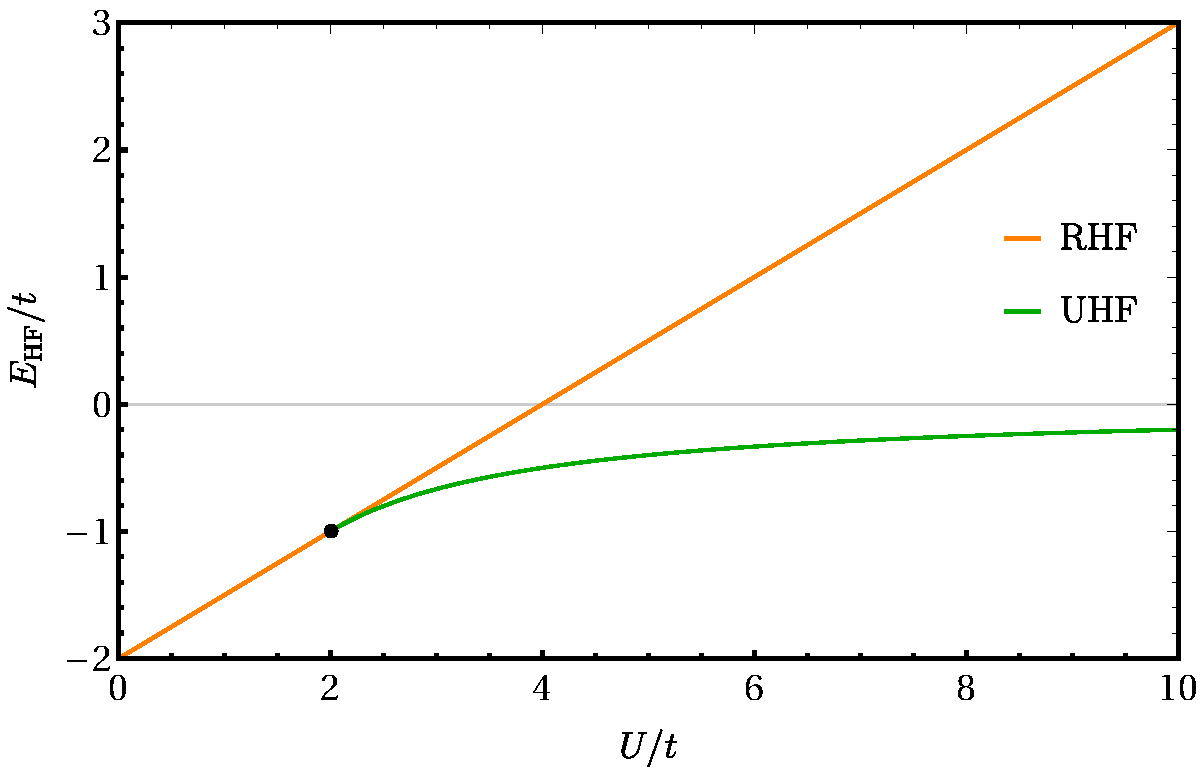
\includegraphics[width=\linewidth]{HF_real.pdf}
    \caption{\label{fig:HF_real}
    RHF and UHF energies as a function of the correlation strength $U/t$. 
    The symmetry-broken UHF solution emerges at the coalescence point $U=2t$ (black dot), often known as the Coulson-Fischer point.}
\end{figure}
%%%%%%%%%%%%%%%%%

In the Hubbard dimer, the UHF energy can be parametrised using two rotation angles $\ta$ and $\tb$ as
\begin{equation}
E_\text{HF}(\ta, \tb) = -t\, \qty( \sin \ta + \sin \tb ) + \frac{U}{2} \qty( 1 + \cos \ta \cos \tb ),
\end{equation}
where we have introduced bonding $\mathcal{B}^{\sigma}$ and anti-bonding $\mathcal{A}^{\sigma}$ molecular orbitals for 
the spin-$\sigma$ electrons as
\begin{subequations}
\begin{align}
    \mathcal{B}^{\sigma} & = \hphantom{-} \cos(\frac{\theta_\sigma}{2}) \Lsi + \sin(\frac{\theta_\sigma}{2}) \Rsi,
	\\
	\mathcal{A}^{\sigma} & = - \sin(\frac{\theta_\sigma}{2}) \Lsi + \cos(\frac{\theta_\sigma}{2}) \Rsi
\end{align}
\end{subequations}
In the weak correlation regime $0 \le U \le 2t$, the angles which minimise the HF energy, 
\ie, $\pdv*{E_\text{HF}}{\theta_\sigma} = 0$, are 
\begin{equation}
	\ta^\text{RHF} = \tb^\text{RHF} = \pi/2,
\end{equation}
giving the symmetry-pure molecular orbitals
\begin{align}
	\mathcal{B}_\text{RHF}^{\sigma} & = \frac{\Lsi + \Rsi}{\sqrt{2}},
	&
	\mathcal{A}_\text{RHF}^{\sigma} & = \frac{\Lsi - \Rsi}{\sqrt{2}},
\end{align}
and the ground-state RHF energy (Fig.~\ref{fig:HF_real})
\begin{equation}
	E_\text{RHF} \equiv E_\text{HF}(\ta^\text{RHF}, \tb^\text{RHF}) = -2t + \frac{U}{2}
\end{equation}
However, in the strongly correlated regime $U>2t$, the closed-shell orbital restriction prevents RHF from 
modelling the correct physics with the two electrons on opposing sites.

%%% FIG 3 (?) %%%
% Analytic Continuation of HF
%%%%%%%%%%%%%%%%%
\begin{figure*}[t]
	\begin{subfigure}{0.49\textwidth}
    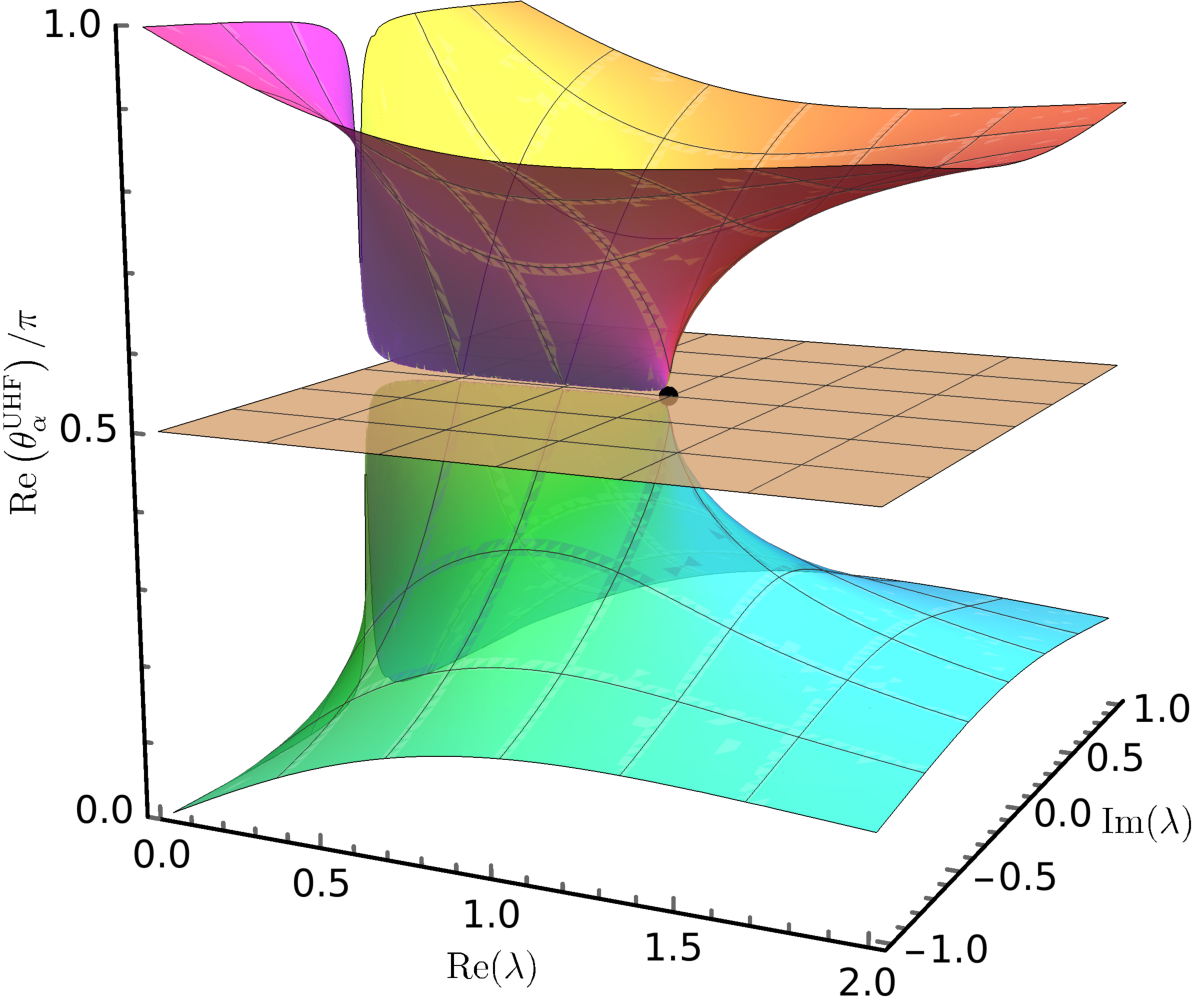
\includegraphics[height=0.65\textwidth,trim={0pt 0pt 0pt -35pt},clip]{HF_cplx_angle}
	\subcaption{\label{subfig:UHF_cplx_angle}}
    \end{subfigure}
	\begin{subfigure}{0.49\textwidth}
	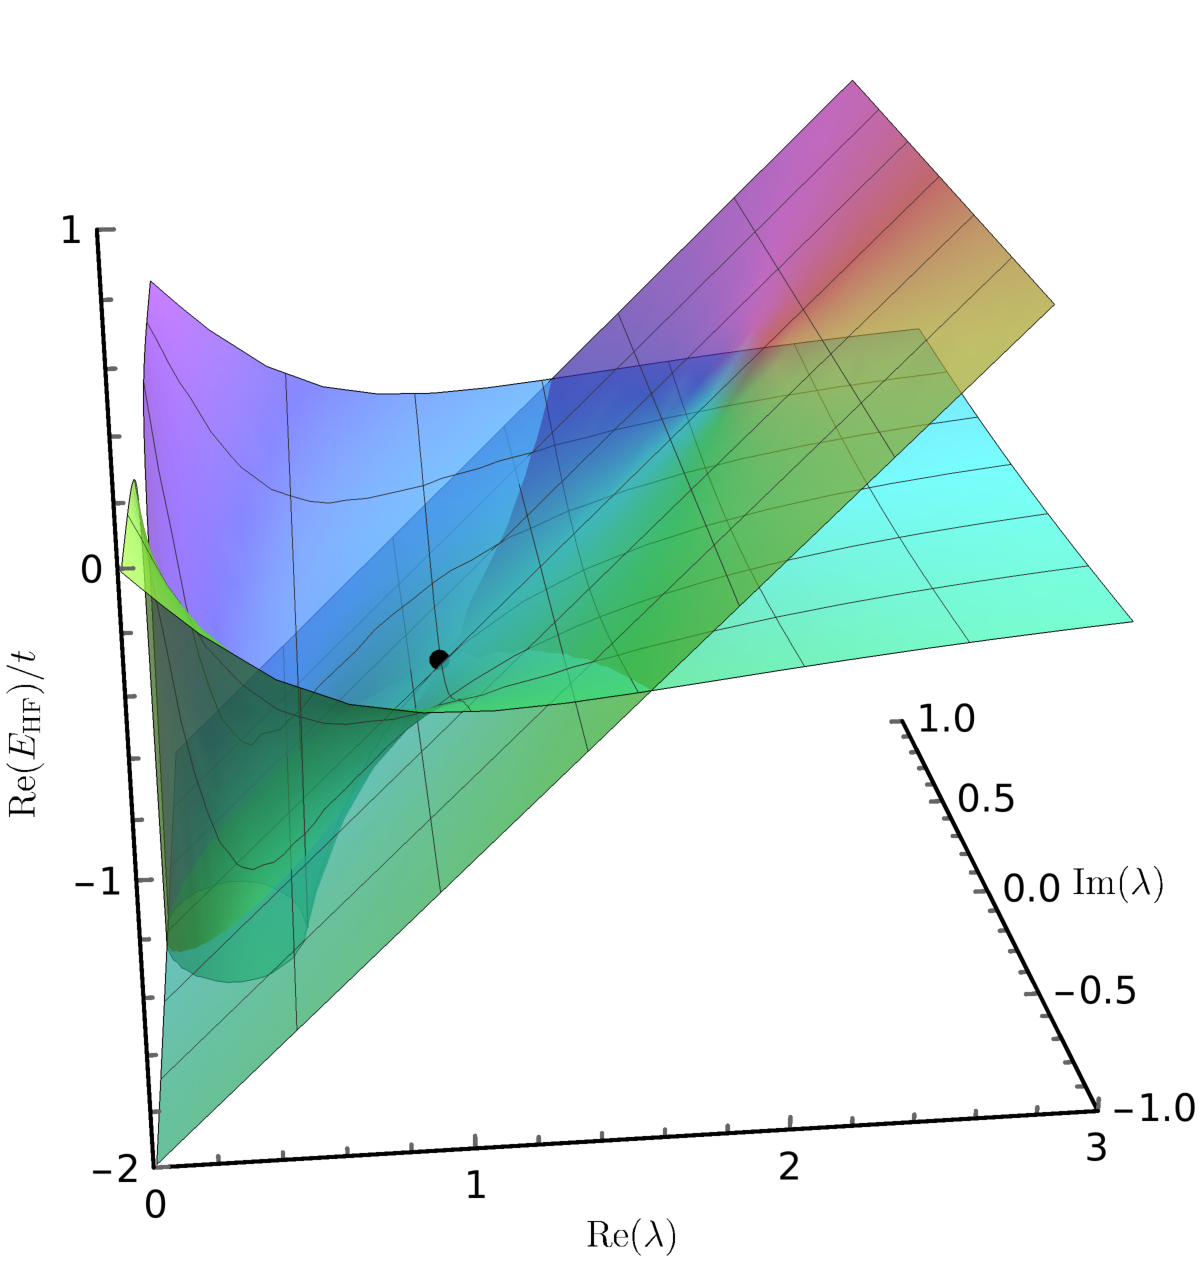
\includegraphics[height=0.65\textwidth]{HF_cplx_energy}
	\subcaption{\label{subfig:UHF_cplx_energy}}
    \end{subfigure}
	\caption{%
    (\subref{subfig:UHF_cplx_angle}) Real component of the UHF angle $\ta^{\text{UHF}}$ for $\lambda \in \bbC$.
    Symmetry-broken solutions correspond to individual sheets and become equivalent at 
    the \textit{quasi}-EP $\lambda_{\text{c}}$ (black dot).
    The RHF solution is independent of $\lambda$, giving the constant plane at $\pi/2$.
    (\subref{subfig:UHF_cplx_energy}) The corresponding HF energy surfaces show a non-analytic 
    point at the \textit{quasi}-EP.
	\label{fig:HF_cplx}}
\end{figure*}
%%%%%%%%%%%%%%%%%

As the on-site repulsion is increased from 0, the HF approximation reaches a critical value at $U=2t$ where a symmetry-broken 
UHF solution appears with a lower energy than the RHF one.
Note that the RHF wave function remains a genuine solution of the HF equations for $U \ge 2t$, but corresponds to a saddle point 
of the HF energy rather than a minimum.
This critical point is analogous to the infamous Coulson--Fischer point identified in the hydrogen dimer.\cite{Coulson_1949}
For $U \ge 2t$, the optimal orbital rotation angles for the UHF orbitals become
\begin{subequations}
\begin{align}
    \ta^\text{UHF} & = \arctan (-\frac{2t}{\sqrt{U^2 - 4t^2}}),
    \label{eq:ta_uhf}
	\\
    \tb^\text{UHF} & = \arctan (+\frac{2t}{\sqrt{U^2 - 4t^2}}),
    \label{eq:tb_uhf}
\end{align}
\end{subequations}
with the corresponding UHF ground-state energy (Fig.~\ref{fig:HF_real})
\begin{equation}
	E_\text{UHF} \equiv E_\text{HF}(\ta^\text{UHF}, \tb^\text{UHF}) = - \frac{2t^2}{U}.
\end{equation}
Time-reversal symmetry dictates that this UHF wave function must be degenerate with its spin-flipped pair, obtained 
by swapping $\ta^{\text{UHF}}$ and $\tb^{\text{UHF}}$ in Eqs.~\eqref{eq:ta_uhf} and \eqref{eq:tb_uhf}.
This type of symmetry breaking is also called a spin-density wave in the physics community as the system
``oscillates'' between the two symmetry-broken configurations. \cite{GiulianiBook}
Symmetry breaking can also occur in RHF theory when a charge-density wave is formed from an oscillation 
between the two closed-shell configurations with both electrons localised on one site or the other.\cite{StuberPaldus,Fukutome_1981}

%============================================================%
\subsection{Self-Consistency as a Perturbation} %OR {Complex adiabatic connection}
%============================================================%

% INTRODUCE PARAMETRISED FOCK HAMILTONIAN
The inherent non-linearity in the Fock eigenvalue problem arises from self-consistency 
in the HF approximation, and is usually solved through an iterative approach.\cite{Roothaan_1951,Hall_1951}
Alternatively, the non-linear terms arising from the Coulomb and exchange operators can 
be considered as a perturbation from the core Hamiltonian \eqref{eq:Hcore} by introducing the
transformation $U \rightarrow \lambda\, U$, giving the parametrised Fock operator 
\begin{equation}
    \Hat{f}(\vb{x} ; \lambda) = \Hat{h}(\vb{x}) + \lambda\, \Hat{v}_\text{HF}(\vb{x}).
\end{equation}
The orbitals in the reference problem $\lambda=0$ correspond to the symmetry-pure eigenfunctions of the one-electron core
Hamiltonian, while self-consistent solutions at $\lambda = 1$ represent the orbitals of the true HF solution.

% INTRODUCE COMPLEX ANALYTIC-CONTINUATION
For real $\lambda$, the self-consistent HF energies at given (real) $U$ and $t$ values
in the Hubbard dimer directly mirror the energies shown in Fig.~\ref{fig:HF_real}, 
with coalesence points at 
\begin{equation}
    \lambda_{\text{c}} = \pm \frac{2t}{U}.
    \label{eq:scaled_fock}
\end{equation}
In contrast, when $\lambda$ becomes complex, the HF equations become non-Hermitian and 
each HF solutions can be analytically continued for all $\lambda$ values using
the holomorphic HF approach.\cite{Hiscock_2014,Burton_2016,Burton_2018}
Remarkably, the coalescence point in this analytic continuation emerges as a 
\textit{quasi}-EP on the real $\lambda$ axis (Fig.~\ref{fig:HF_cplx}), where
the different HF solutions become equivalent but not self-orthogonal.\cite{Burton_2019}
By analogy with perturbation theory, the regime where this \textit{quasi}-EP occurs 
within $\lambda_{\text{c}} \le 1$ can be interpreted as an indication that 
the symmetry-pure reference orbitals no longer provide a qualitatively 
accurate representation for the true HF ground state at $\lambda = 1$.
For example, in the Hubbard dimer with $U > 2t$, one finds $\lambda_{\text{c}} < 1$ and the symmetry-pure orbitals
do not provide a good representation of the HF ground state.
In contrast, $U < 2t$ yields $\lambda_{\text{c}} > 1$ and corresponds to
the regime where the HF ground state is correctly represented by symmetry-pure orbitals.

% COMPLEX ADIABATIC CONNECTION
We have recently shown that the complex scaled Fock operator Eq.~\eqref{eq:scaled_fock}
also allows states of different symmetries to be interconverted by following a well-defined
contour in the complex $\lambda$-plane.\cite{Burton_2019}
In particular, by slowly varying $\lambda$ in a similar (yet different) manner
to an adiabatic connection in density-functional theory,\cite{Langreth_1975,Gunnarsson_1976,Zhang_2004} 
a ground-state wave function can be ``morphed'' into an excited-state wave function 
via a stationary path of HF solutions.
This novel approach to identifying excited-state wave functions demonstrates the fundamental 
role of \textit{quasi}-EPs in determining the behaviour of the HF approximation.

%\titou{In a recent paper, \cite{Burton_2019} using holomorphic Hartree-Fock (h-HF) \cite{Hiscock_2014,Burton_2018,Burton_2016} as an analytic continuation of conventional HF theory, we have demonstrated, on a simple model, that one can interconvert states of different symmetries and natures by following well-defined contours in the complex $\lambda$-plane, where $\lambda$ is the strength of the electron-electron interaction (see Fig.~\ref{fig:iAC}).
%In particular, by slowly varying $\lambda$ in a similar (yet different) manner to an adiabatic connection in density-functional theory, \cite{Langreth_1975,Gunnarsson_1976,Zhang_2004} one can ``morph'' a ground-state wave function into an excited-state wave function via a stationary path of HF solutions. \cite{Seidl_2018}
%In such a way, we could obtain a doubly-excited state wave function starting from the ground state wave function, a process which is not as easy as one might think. \cite{Gilbert_2008,Thom_2008,Shea_2018}
%One of the fundamental discovery we made was that Coulson-Fischer points (where multiple symmetry-broken solutions coalesce) play a central role and can be classified as \textit{quasi}-exceptional points, as the wave functions do not become self-orthogonal.
%The findings reported in Ref.~\onlinecite{Burton_2019} represent the very first study of non-Hermitian quantum mechanics for the exploration of multiple solutions at the HF level. 
%It perfectly illustrates the deeper topology of electronic states revealed using a complex-scaled electron-electron interaction.
%Through the introduction of non-Hermiticity, we have provided a more general framework in which the complex and diverse characteristics of multiple solutions can be explored and understood.}

%%%%%%%%%%%%%%%%%%%%%%%%%%%%%%%%%%%%%%%%%%%%%%%
\section{M{\o}ller--Plesset Perturbation Theory in the Complex Plane}
\label{sec:MP}
%%%%%%%%%%%%%%%%%%%%%%%%%%%%%%%%%%%%%%%%%%%%%%%


%=====================================================%
\subsection{Background Theory}
%=====================================================%

In electronic structure, the HF Hamiltonian \eqref{eq:HFHamiltonian} is often used as the zeroth-order Hamiltonian
to define M\o{}ller--Plesset (MP) perturbation theory.\cite{Moller_1934}
This approach can recover a large proportion of the electron correlation energy,\cite{Lowdin_1955a,Lowdin_1955b,Lowdin_1955c} 
and provides the foundation for numerous post-HF approximations.
With the MP partitioning, the parametrised perturbation Hamiltonian becomes
\begin{multline}\label{eq:MPHamiltonian}
    \hH(\lambda) =   
     \sum_{i}^{N} \qty[ - \frac{\grad_i^2}{2} - \sum_{A}^{M} \frac{Z_A}{\abs{\vb{r}_i-\vb{R}_A}} ]
    \\
    + (1-\lambda) \sum_{i}^{N} v^{\text{HF}}(\vb{x}_i)
    + \lambda\sum_{i<j}^{N}\frac{1}{\abs{\vb{r}_i-\vb{r}_j}}.
\end{multline}
Any set of orbitals can be used to define the HF Hamiltonian, although either the RHF or UHF orbitals are usually chosen to 
define the RMP or UMP series respectively.
The MP energy at a given order $n$ (\ie, MP$n$) is then defined as
\begin{equation}
	E_{\text{MP}n}= \sum_{k=0}^n E_{\text{MP}}^{(k)},
\end{equation}
where $E_{\text{MP}}^{(k)}$ is the $k$th-order MP correction and 
\begin{equation}
E_{\text{MP1}} =  E_{\text{MP}}^{(0)} + E_{\text{MP}}^{(1)} = E_\text{HF}.
\end{equation}
The second-order MP2 energy is given by
\begin{equation}\label{eq:EMP2}
	E_{\text{MP2}} = \frac{1}{4} \sum_{ij} \sum_{ab} \frac{\abs{\mel{ij}{}{ab}}^2}{\epsilon_i + \epsilon_j - \epsilon_a - \epsilon_b},
\end{equation}
where $\mel{pq}{}{rs} = \braket{pq}{rs} - \braket{pq}{sr}$ are the anti-symmetrised two-electron integrals
in the molecular spin-orbital basis\cite{Gill_1994}
\begin{equation}
	\braket{pq}{rs} 
    = \iint \dd\vb{x}_1\dd\vb{x}_2
    \frac{\phi^{*}_p(\vb{x}_1)\phi^{*}_q(\vb{x}_2)\phi^{\vphantom{*}}_r(\vb{x}_1)\phi^{\vphantom{*}}_s(\vb{x}_2)}%
      {\abs{\vb{r}_1 - \vb{r}_2}}.
\end{equation}

While most practical calculations generally consider only the MP2 or MP3 approximations, higher order terms can 
easily be computed to understand the convergence of the MP$n$ series.\cite{Handy_1985}
\textit{A priori}, there is no guarantee that this series will provide the smooth convergence that is desirable for a
systematically improvable theory.
In fact, when the reference HF wave function is a poor approximation to the exact wave function, 
for example in multi-configurational systems, MP theory can yield highly oscillatory, 
slowly convergent, or catastrophically divergent results.\cite{Gill_1986,Gill_1988,Handy_1985,Lepetit_1988,Leininger_2000}
Furthermore, the convergence properties of the MP series can depend strongly on the choice of restricted or
unrestricted reference orbitals.

% HGAB: I don't think this parapgrah tells us anything we haven't discussed before
%A convenient way to investigate the convergence properties of the MP series is to analytically continue the coupling parameter $\lambda$ into the complex variable. 
%By doing so, the Hamiltonian and the energy become complex-valued functions of $\lambda$, 
%and the energy becomes a multivalued function on $K$ Riemann sheets (where $K$ is the number of basis functions).
%As mentioned above, by searching the singularities of the function $E(\lambda)$, one can get information on the convergence properties of the MP series. 
%These singularities of the energy function are exactly the EPs connecting the electronic states as mentioned in Sec.~\ref{sec:intro}. 
%The direct computation of the terms of the series is quite manageable up to fourth order in perturbation, while the fifth and sixth order in perturbation can still be obtained but at a rather high cost. \cite{JensenBook}
%In order to better understand the behaviour of the MP series and how it is connected to the singularity structure, we have to access high-order terms. 
%For small systems, one can access the whole terms of the series using full configuration interaction (FCI). 
%If the Hamiltonian $H(\lambda)$ is diagonalized in the FCI space, one gets the exact energies (in this finite Hilbert space) and the Taylor expansion with respect to $\lambda$ allows to access the MP perturbation series at any order.


Although practically convenient for electronic structure calculations, the MP partitioning is not 
the only possibility and alternative partitionings have been considered including: %proposed in the literature:
i) the Epstein-Nesbet (EN) partitioning which consists in taking the diagonal elements of $\hH$ as the zeroth-order Hamiltonian. \cite{Nesbet_1955,Epstein_1926} 
%Hence, the off-diagonal elements of $\hH$ are the perturbation operator,
ii) the weak correlation partitioning in which the one-electron part is consider as the unperturbed Hamiltonian $\hH^{(0)}$ and the two-electron part is the perturbation operator $\hV$, and 
iii) the strong coupling partitioning where the two operators are inverted compared to the weak correlation partitioning. \cite{Seidl_2018}
While an in-depth comparison of these different approaches can offer insight into 
their relative strengths and weaknesses for various situations, we will restrict our current discussion
to the convergence properties of the MP expansion.

%=====================================================%
\subsection{Early Investigations into M{\o}ller--Plesset Convergence} % in Molecular Systems}
%=====================================================%

% GENERAL DESIRE FOR WELL-BEHAVED CONVERGENCE AND LOW-ORDER TERMS
 Among the most desirable properties of any electronic structure technique is the existence of 
a systematic route to increasingly accurate energies. 
In the context of MP theory, one would like a monotonic convergence of the perturbation
series towards the exact energy such that the accuracy increases as each term in the series is added.
If such well-behaved convergence can be established, then our ability to compute individual 
terms in the series becomes the only barrier to computing the exact correlation in a finite basis set.
Unfortunately, the computational scaling of each term in the MP series increases with the perturbation
order, and practical calculations must rely on fast convergence
to obtain high-accuracy results using only the lowest order terms.

% INITIAL POSITIVITY AROUND THE CONVERGENCE PROPERTIES AND EARLY WORK SCOPE
MP theory was first introduced to quantum chemistry through the pioneering
works of Bartlett \etal\ in the context of many-body perturbation theory,\cite{Bartlett_1975}
and Pople and co-workers in the context of determinantal expansions.\cite{Pople_1976,Pople_1978}
Early implementations were restricted to the fourth-order MP4 approach that was considered
to offer state-of-the-art quantitative accuracy.\cite{Pople_1978,Krishnan_1980}
However, it was quickly realised that the MP series often demonstrated very slow, oscillatory, 
or erratic convergence, with the UMP series showing particularly slow convergence.\cite{Laidig_1985,Knowles_1985,Handy_1985}
For example, RMP5 is worse than RMP4 for predicting the homolytic barrier fission of \ce{He2^2+} using a minimal basis set, 
while the UMP series monotonically converges but becomes increasingly slow beyond UMP5.\cite{Gill_1986}
The first examples of divergent MP series were observed in the \ce{N2} and \ce{F2} 
diatomics, where low-order RMP and UMP expansions give qualitatively wrong binding curves.\cite{Laidig_1987} 

% SLOW UMP CONVERGENCE AND SPIN CONTAMINATION
The divergence of RMP expansions for stretched bonds can be easily understood from two perspectives.\cite{Gill_1988a}
Firstly, the exact wave function becomes increasingly multi-configurational as the bond is stretched, and the 
HF wave function no longer provides a qualitatively correct reference for the perturbation expansion.
Secondly, the energy gap between the bonding and anitbonding orbitals associated with the stretch becomes
increasingly small at larger bond lengths, leading to a divergence in the Rayleigh--Schr\"odinger perturbation
expansion Eq.~\eqref{eq:EMP2}.
In contrast, the origin of slow UMP convergence is less obvious as the reference UHF energy remains
qualitatively correct at large bond lengths and the orbital degeneracy is avoided.
Furthermore, this slow convergence can also be observed in molecules with a UHF ground state at the equilibrium
geometry (\eg, \ce{CN-}), suggesting a more fundamental link with spin-contamination 
in the reference wave function.\cite{Nobes_1987}

Using the UHF framework allows the singlet ground state wave function to mix with triplet wave functions, 
leading to spin contamination where the wave function is no longer an eigenfunction of the $\Hat{\cS}^2$ operator.
The link between slow UMP convergence and this spin-contamination was first systematically investigated
by Gill \etal\ using the minimal basis \ce{H2} model.\cite{Gill_1988}
In this work, the authors compared the UMP series with the exact RHF- and UHF-based FCI expansions
and identified that the slow UMP convergence arises from its failure to correctly predict the amplitude of the
low-lying double excitation.
This erroneous description of the double excitation amplitude has the same origin as the spin-contamination in the reference
UHF wave function, creating the first direct link between spin-contamination and slow UMP convergence.\cite{Gill_1988}
Lepetit \etal\ later analysed the difference between perturbation convergence using the unrestricted MP 
and EN partitionings. \cite{Lepetit_1988}
They argued that the slow UMP convergence for stretched molecules arises from 
(i) the fact that the MP denominator (see Eq.~\ref{eq:EMP2})
tends to a constant value instead of vanishing, and (ii) the slow convergence of contributions from the 
singly-excited configurations that strongly couple to the doubly-excited configurations and first
appear at fourth-order.\cite{Lepetit_1988}
Drawing these ideas together, we believe that slow UMP convergence occurs because the single excitations must focus on removing
spin-contamination from the reference wave function, limiting their ability to fine-tune the amplitudes of the higher 
excitations that capture the correlation energy.

% SPIN-PROJECTION SCHEMES
A number of spin-projected extensions have been derived to reduce spin-contamination in the wave function
and overcome the slow UMP convergence.
Early versions of these theories, introduced by Schlegel \cite{Schlegel_1986, Schlegel_1988} or 
Knowles and Handy,\cite{Knowles_1988a,Knowles_1988b} exploited the ``projection-after-variation'' philosophy,
where the spin-projection is applied directly to the UMP expansion.
These methods succeeded in accelerating the convergence of the projected MP series and were 
considered as highly effective methods for capturing the electron correlation at low computational cost.\cite{Knowles_1988b}
However, the use of projection-after-variation leads to gradient discontinuities in the vicinity of the UHF symmetry-breaking point,
and can result in spurious minima along a molecular binding curve.\cite{Schlegel_1986,Knowles_1988a}
More recent formulations of spin-projected perturbations theories have considered the  
``variation-after-projection'' framework using alternative definitions of the reference 
Hamiltonian.\cite{Tsuchimochi_2014,Tsuchimochi_2019}
These methods yield more accurate spin-pure energies without 
gradient discontinuities or spurious minima.

%When one relies on MP perturbation theory (and more generally on any perturbative partitioning), it would be reasonable to ask for a systematic improvement of the energy with respect to the perturbative order, \ie, one would expect that the more terms of the perturbative series one can compute, the closer the result from the exact energy.
%In other words, one would like a monotonic convergence of the MP series. Assuming this, the only limiting process to get the exact correlation energy (in a finite basis set) would be our ability to compute the terms of this perturbation series.
%Unfortunately this is not as easy as one might think because i) the terms of the perturbative series become rapidly computationally cumbersome, and ii) erratic behaviour of the perturbative coefficients are not uncommon. 
%For example, in the late 80's, Gill and Radom reported deceptive and slow convergences in stretched systems \cite{Gill_1986,Gill_1988} (see also Refs.~\onlinecite{Handy_1985,Lepetit_1988}). 
%In Ref.~\onlinecite{Gill_1986}, the authors showed that the RMP series is convergent, yet oscillatory which is far from being convenient if one is only able to compute the first few terms of the expansion.
%For example, in the case of the barrier to homolytic fission of \ce{He2^2+} in a minimal basis set, RMP5 is worse than RMP4 (see Fig.~2 in Ref.~\onlinecite{Gill_1986}).
%On the other hand, the UMP series is monotonically convergent after UMP5 but very slowly . 
%Thus, one cannot practically use it for systems where only the first terms are computationally accessible.

%When a bond is stretched, in most cases the exact wave function becomes more and more of multi-reference nature. 
%Yet, the HF wave function is restricted to be a single Slater determinant.
%It is then inappropriate to model (even qualitatively) stretched systems. 
%Nevertheless, as explained in Sec.~\ref{sec:HF} and illustrated in Sec.~\ref{sec:HF_hubbard}, the HF wave function can undergo symmetry breaking to lower its energy by sacrificing one of the symmetry of the exact wave function in the process (see also the pedagogical example of \ce{H2} in Ref.~\onlinecite{SzaboBook}). 
%One could then potentially claim that the RMP series exhibits deceptive convergence properties as the RHF Slater determinant is a poor approximation of the exact wave function for stretched system. 
%However, as illustrated above, even in the unrestricted formalism which clearly represents a better description of a stretched system, the UMP series does not have the smooth and rapidly convergent behaviour that one would wish for. 
%The reasons behind this ambiguous behaviour are further explained below.

%In the unrestricted framework the singlet ground state wave function is allowed to mix with triplet wave functions, leading to the so-called spin contamination issue. Gill \textit{et al.}~highlighted the link between slow convergence of the UMP series and spin contamination for \ce{H2} in a minimal basis. \cite{Gill_1988}
%Handy and coworkers reported the same behaviour of the UMP series (oscillatory and slowly monotonically convergent) in stretched \ce{H2O} and \ce{NH2}. \cite{Handy_1985} Lepetit \textit{et al.}~analysed the difference between the MP and EN partitioning for the UHF reference. \cite{Lepetit_1988} 
%They concluded that the slow convergence of the UMP series is due to i) the fact that the MP denominator (see Eq.~\ref{eq:EMP2}) tends to a constant instead of vanishing, and ii) the lack of the singly-excited configurations (which only appears at fourth order) that strongly couple to the doubly-excited configurations.
%We believe that this divergent behaviour might therefore be attributed to the need for the single excitations to focus on correcting the structure of the reference orbitals rather than capturing the correlation energy. 

%Cremer and He analysed 29 atomic and molecular systems at the FCI level \cite{Cremer_1996} and grouped them in two classes: i) the \textit{class A} systems where one observes a monotonic convergence \titou{of the RMP series?} to the FCI energy, and ii) the \textit{class B} systems for which convergence is erratic after initial oscillations. 
%Their system set contains stretched molecules as well as molecules at their equilibrium geometry for various basis sets. 
%They highlighted that \cite{Cremer_1996}
%\textit{``Class A systems are characterised by electronic structures with well-separated electron pairs while class B systems are characterized by electronic structures with electron clustering in one or more regions.''}
%Moreover, they analysed the contribution of the triple (T) excitations to the MP4, MP5 and MP6 energies next to the single, double and quadruple (SDQ) excitations contribution.
%They showed that class A systems have very little contribution from the triple excitations and that most of the correlation energy is due to pair correlation. 
%On the other hand, class B systems have an important contribution from the triple excitations which alternates in sign resulting in an oscillation of the total correlation energy.
%This observation on the contribution to the MP$n$ energy corroborates the electronic structure discussed above.
%As one can only compute the first terms of the MP series, a smart way of getting more accurate results is to use extrapolation formula, \ie, estimating the limit of the series with only few terms. 
%Cremer and He proved that using specific extrapolation formulas of the MP series for class A and class B systems improves the precision of the results compared to the formula used without resorting to classes. \cite{Cremer_1996}
%The mean absolute deviation taking the FCI correlation energies as reference is $0.3$ millihartree with the class-specific formula whereas the deviation increases to 12 millihartree using the general formula.  
%Even if there were still shaded areas in their analysis and that their classification was incomplete, the work of Ref.~\onlinecite{Cremer_1996} clearly evidenced that understanding the origin of the different modes of convergence could potentially lead to a more rationalised use of MP perturbation theory and, hence, to more accurate correlation energy estimates.


%==========================================%
\subsection{Spin-Contamination in the Hubbard Dimer}
%==========================================%

%%% FIG 2 %%%
\begin{figure*}
	\begin{subfigure}{0.32\textwidth}
	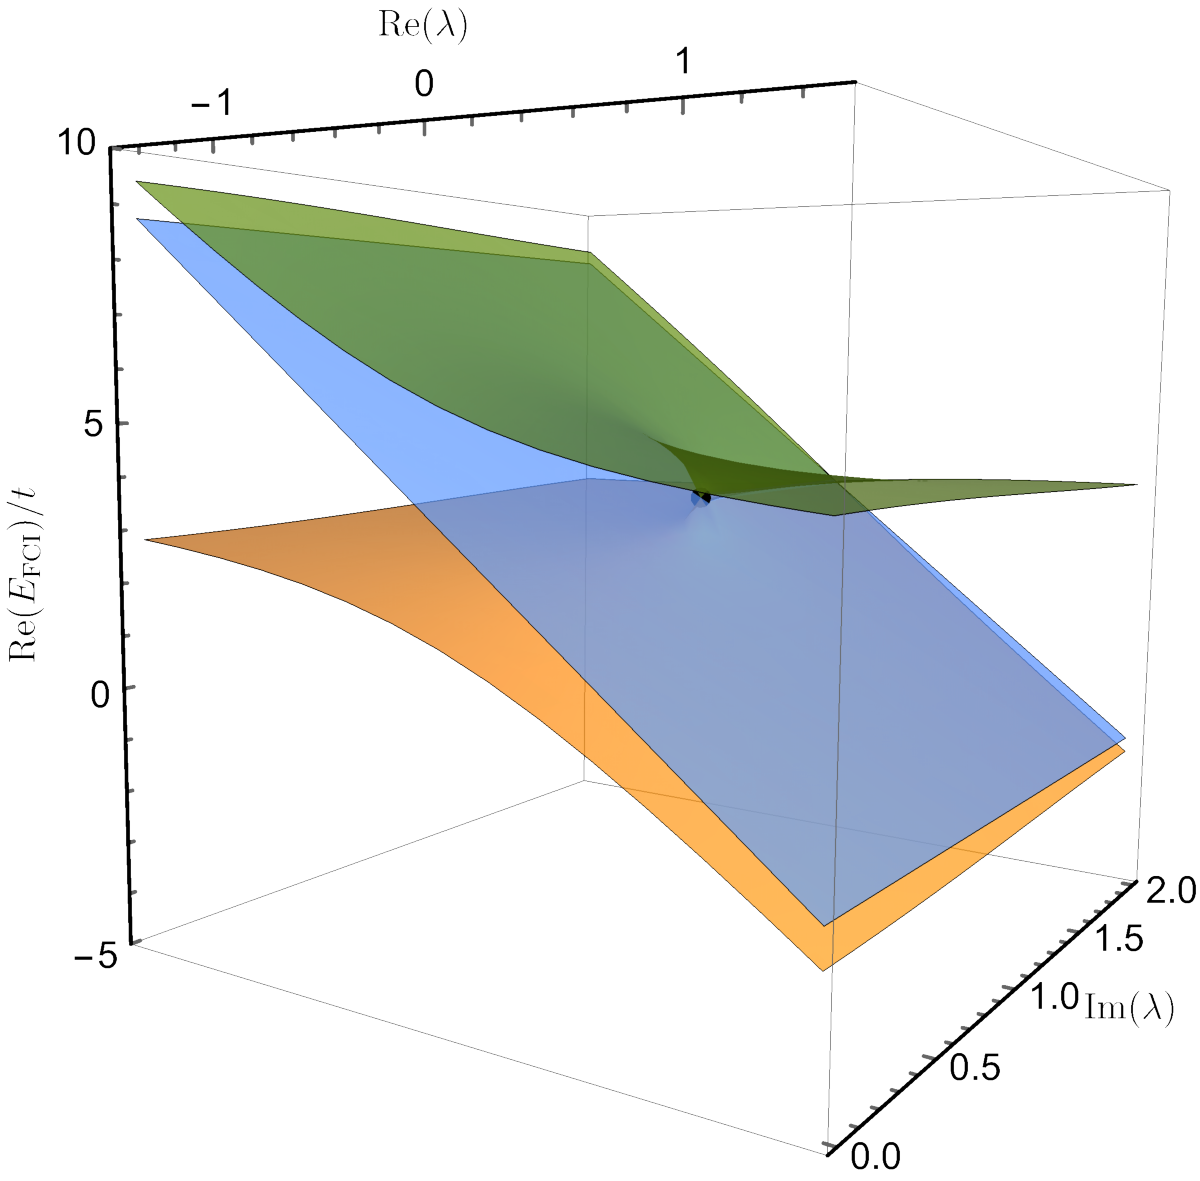
\includegraphics[height=0.75\textwidth]{fig2a}	
		\subcaption{\label{subfig:RMP_3.5} $U/t = 3.5$}
    \end{subfigure}
    %
    \begin{subfigure}{0.32\textwidth}
	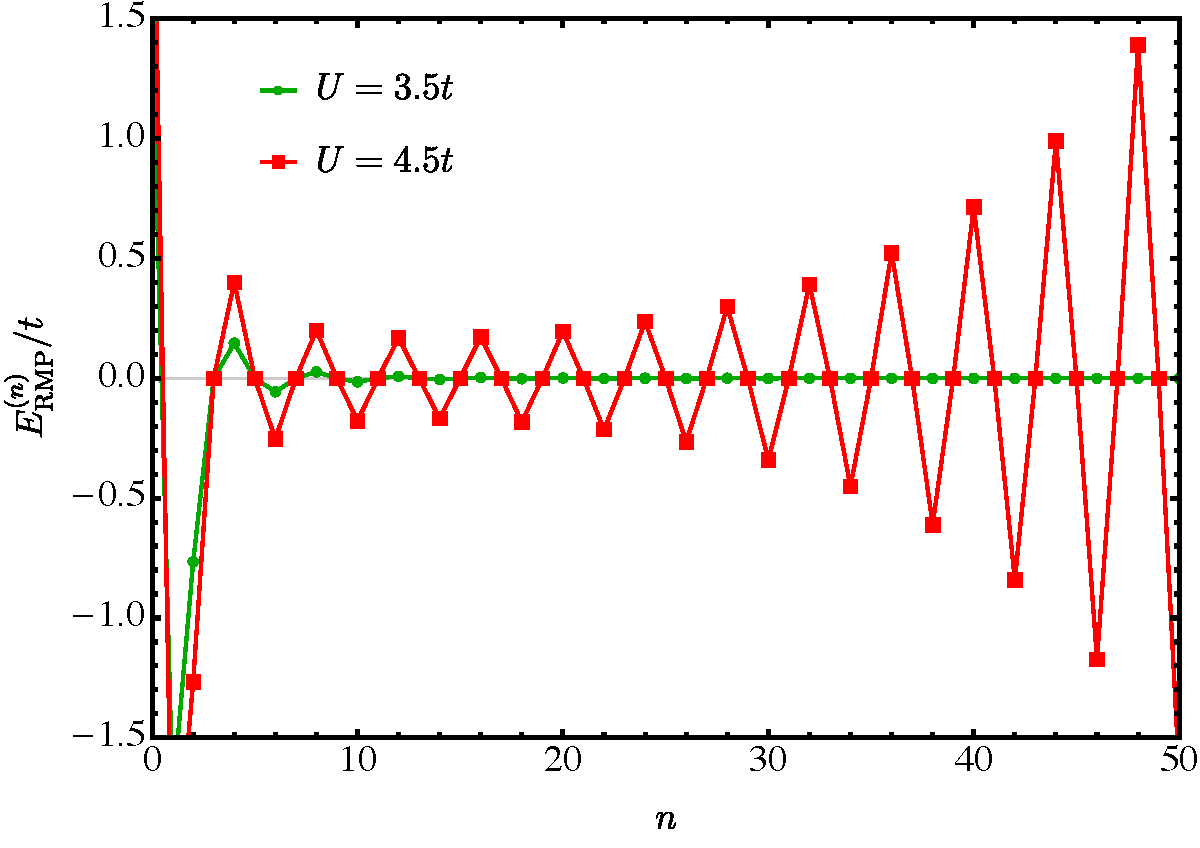
\includegraphics[height=0.75\textwidth]{fig2b}
		\subcaption{\label{subfig:RMP_cvg}}
    \end{subfigure}
    %
    \begin{subfigure}{0.32\textwidth}
	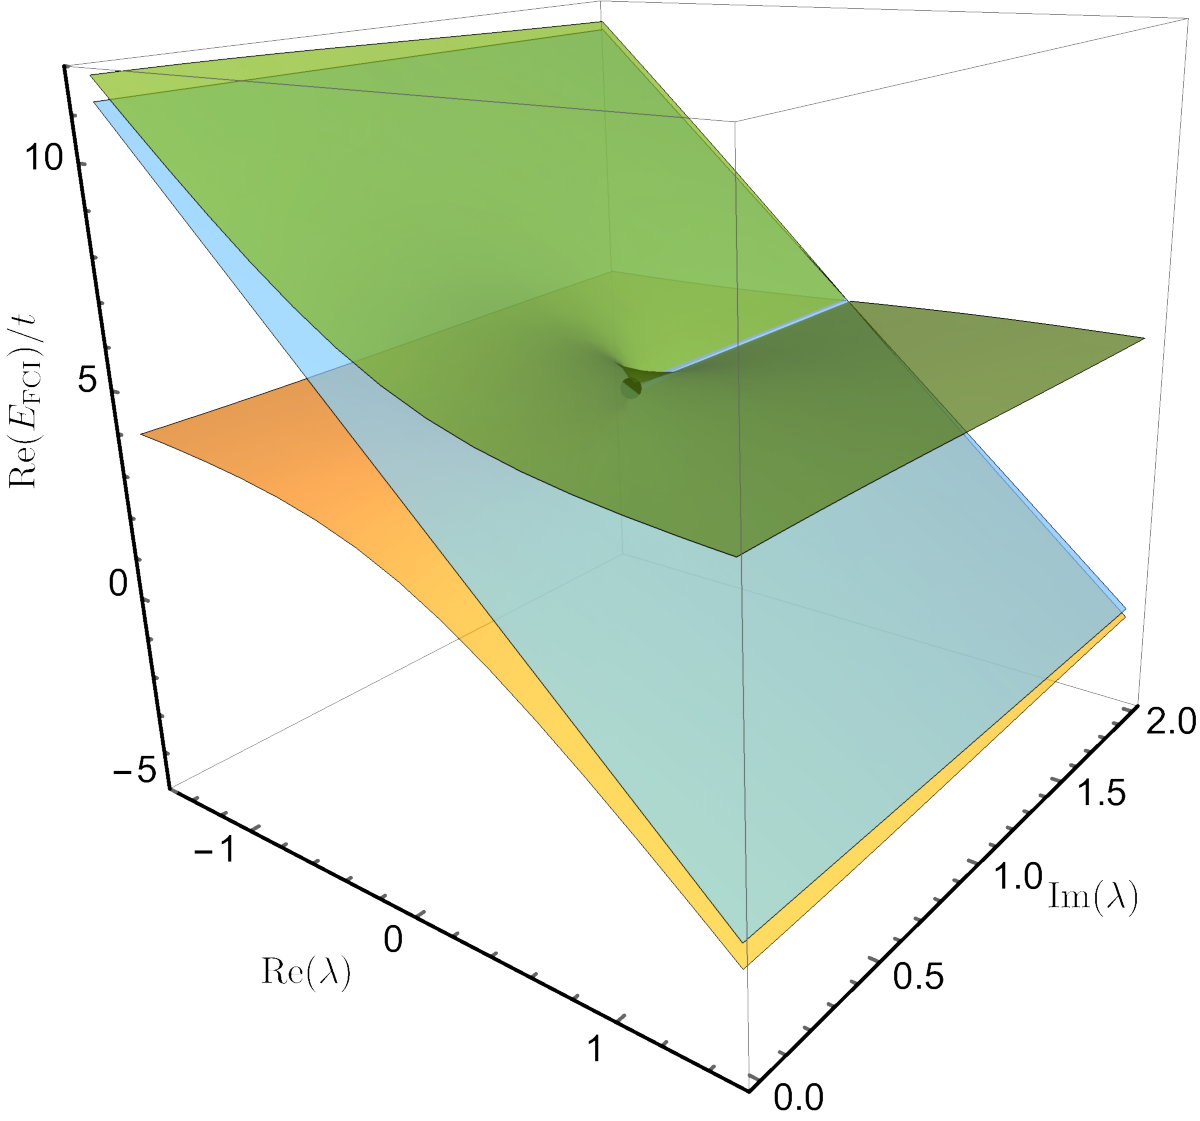
\includegraphics[height=0.75\textwidth]{fig2c}	
		\subcaption{\label{subfig:RMP_4.5} $U/t = 4.5$}
    \end{subfigure}
	\caption{
	Convergence of the RMP series as a function of the perturbation order $n$ for the Hubbard dimer at $U/t = 3.5$ (where $r_c > 1$) and $4.5$ (where $r_c < 1$).
	The Riemann surfaces associated with the exact energies of the RMP Hamiltonian \eqref{eq:H_RMP} are also represented for these two values of $U/t$ as functions of $\lambda$. 
	\label{fig:RMP}}
\end{figure*}

The behaviour of the RMP and UMP series observed in \ce{H2} can also be illustrated by considering
the analytic Hubbard dimer with a complex-valued perturbation strength.
In this system, the stretching of the \ce{H\bond{-}H} bond is directly mirrored by an increase in the electron correlation $U/t$.
Using the ground-state RHF reference orbitals leads to the parametrised RMP Hamiltonian
\begin{widetext}
\begin{equation}
\label{eq:H_RMP}
\bH_\text{RMP}\qty(\lambda) = 
	\begin{pmatrix}
		-2t + U - \lambda U/2	&	0					&	0					&	\lambda U/2	\\
		0						&	U - \lambda U/2 	&	\lambda U/2			&	0	\\
		0						&	\lambda U/2			&	U - \lambda U/2 	&	0	\\
		\lambda U/2 			&	0 					&	0					&	2t + U - \lambda U/2	\\
	\end{pmatrix},
\end{equation}
\end{widetext}
which yields the ground-state energy 
\begin{equation}
	\label{eq:E0MP}
	E_{-}(\lambda) = U - \frac{\lambda U}{2} - \frac{1}{2} \sqrt{(4t)^2 + \lambda ^2 U^2}.
\end{equation}
From this expression, the EPs can be identified as $\lep = \pm \i 4t / U$,
giving the radius of convergence
\begin{equation}
    \rc = \abs{\frac{4t}{U}}.
\end{equation}
Remarkably, these EPs are identical to the exact EPs discussed in Sec.~\ref{sec:example}.
The Taylor expansion of the RMP energy can then be evaluated to obtain the $k$th-order MP correction
\begin{equation}
	E_\text{RMP}^{(k)} = U \delta_{0,k} - \frac{1}{2} \frac{U^k}{(4t)^{k-1}} \mqty( 1/2 \\ k/2).
\end{equation}
%with 
%\begin{equation}
%	E_{\text{MP}n}(\lambda) = \sum_{k=0}^n E_\text{MP}^{(k)} \lambda^k.
%\end{equation}
 
%%%%%%%%%%%%%%%%%%%%%%%%%%%%%
% RADIUS OF CONVERGENCE PLOTS
%%%%%%%%%%%%%%%%%%%%%%%%%%%%%
\begin{figure}[htb]
	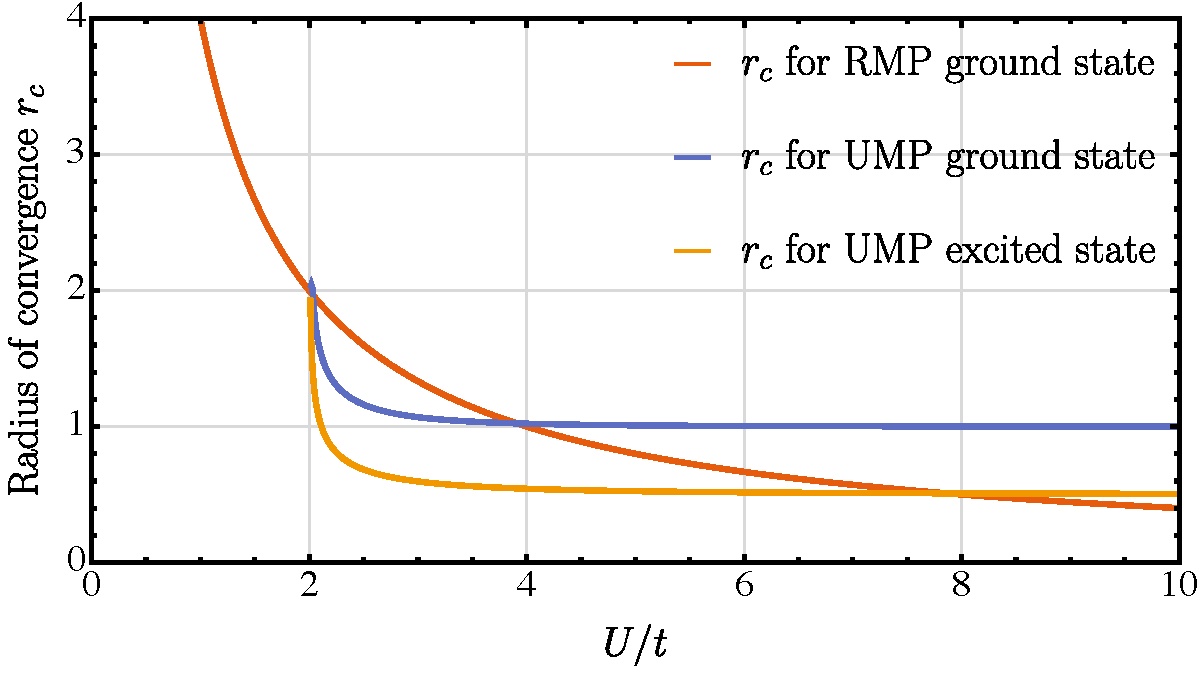
\includegraphics[width=\linewidth]{RadConv}
	\caption{
	Radius of convergence $r_c$ for the RMP ground state (red), the UMP ground state (blue), and the UMP excited state (orange) 
    series as functions of the ratio $U/t$.
	\label{fig:RadConv}}
\end{figure}
%%%%%%%%%%%%%%%%%%%%%%%%%%%%%

The RMP series is convergent for $U = 3.5\,t$ with $\rc > 1$, as illustrated for the individual terms at each order
of perturbation in Fig.~\ref{subfig:RMP_cvg}.
In contrast, for $U = 4.5t$ one finds $\rc < 1$, and the RMP series becomes divergent.
The corresponding Riemann surfaces for $U = 3.5\,t$ and $4.5\,t$ are shown in Figs.~\ref{subfig:RMP_3.5} and 
\ref{subfig:RMP_4.5}, respectively, with the single EP at $\lep$ (black dot) and the radius of convergence indicated
by the vertical cylinder of unit radius.
For the divergent case, the $\lep$ lies inside this cylinder of convergence, while in the convergent case $\lep$ lies
outside this cylinder.
In both cases, the EP connects the ground state with the doubly-excited state, and thus the convergence behaviour
for the two states using the ground-state RHF orbitals is identical.
% HGAB: This cannot be relevant here as the single-excitations don't couple to either ground or excited state.
%The convergent and divergent series start to differ at fourth order, corresponding to the lowest-order contribution
%%from the single excitations.\cite{Lepetit_1988}

%%% FIG 3 %%%
\begin{figure*}
	\begin{subfigure}{0.32\textwidth}
	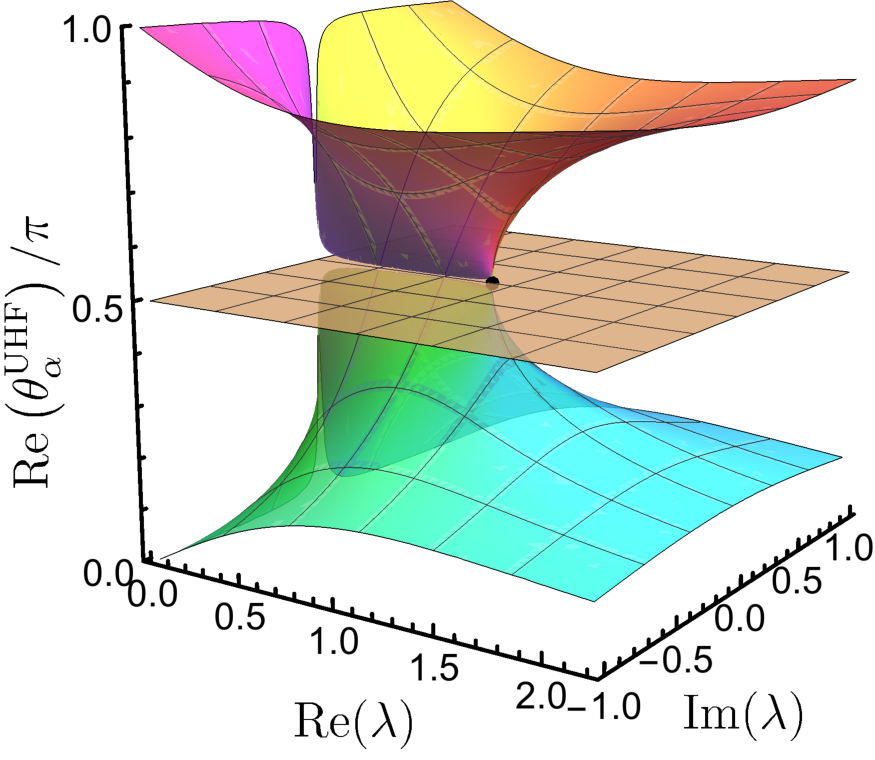
\includegraphics[height=0.75\textwidth]{fig3a}	
		\subcaption{\label{subfig:UMP_3} $U/t = 3$}
    \end{subfigure}
    %
    \begin{subfigure}{0.32\textwidth}
	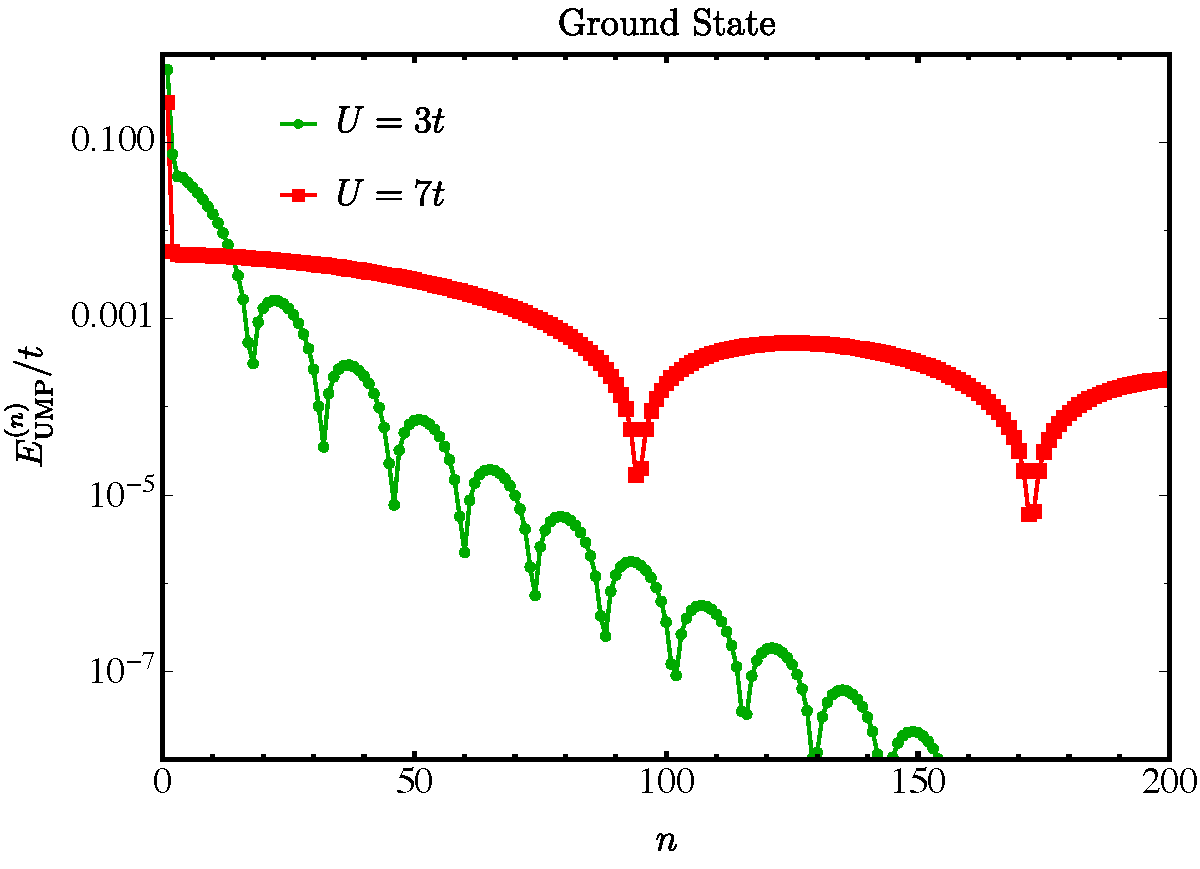
\includegraphics[height=0.75\textwidth]{fig3b}
		\subcaption{\label{subfig:UMP_cvg}}
    \end{subfigure}
    %
    \begin{subfigure}{0.32\textwidth}
	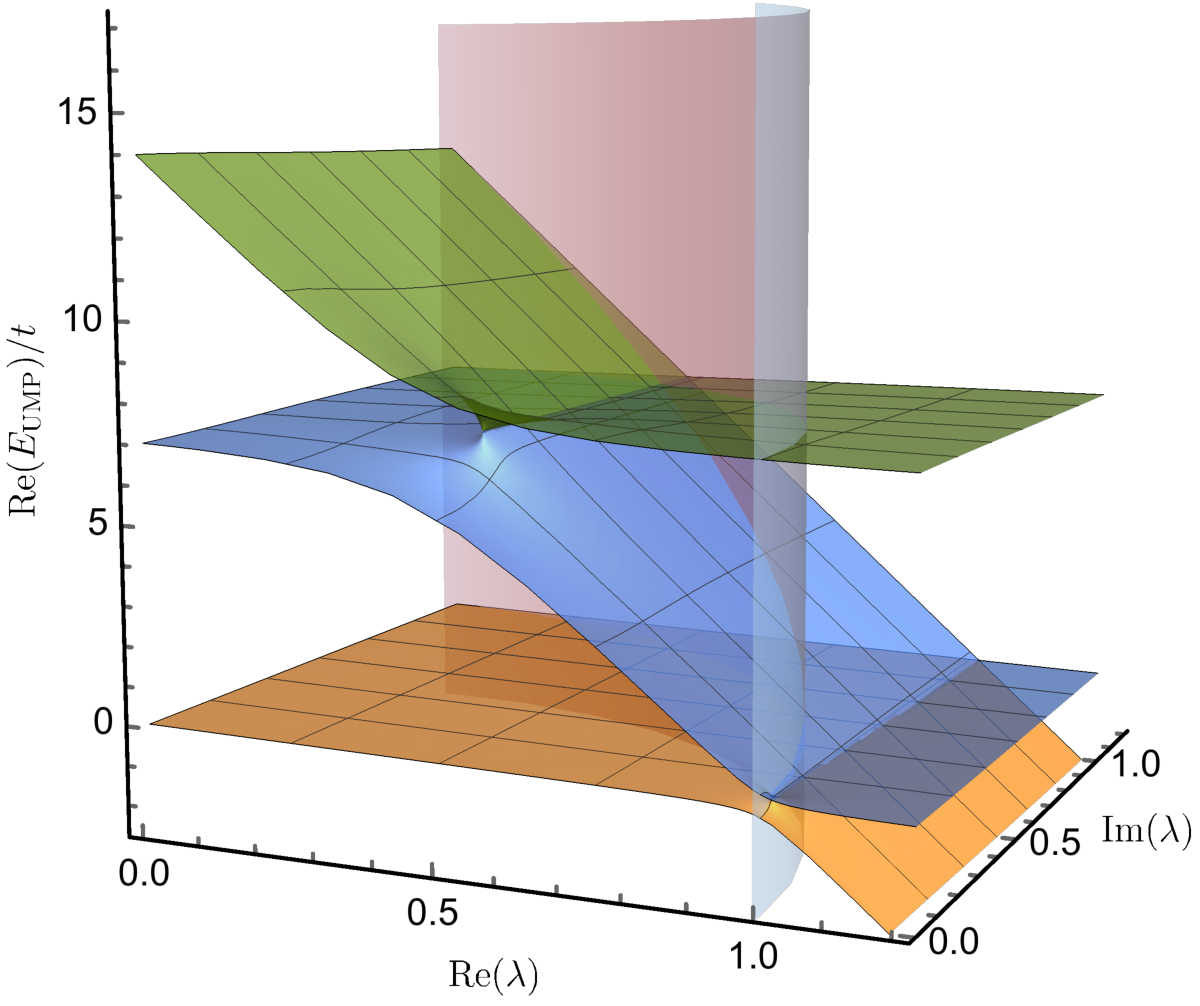
\includegraphics[height=0.75\textwidth]{fig3c}	
		\subcaption{\label{subfig:UMP_7} $U/t = 7$}
    \end{subfigure}	\caption{
	Convergence of the UMP series as a function of the perturbation order $n$ for the Hubbard dimer at $U/t = 3$ and $7$.
	The Riemann surfaces associated with the exact energies of the UMP Hamiltonian \eqref{eq:H_UMP} are also represented for these two values of $U/t$ as functions of $\lambda$.
	\label{fig:UMP}}
\end{figure*}

The behaviour of the UMP series is more subtle than the RMP series as the spin-contamination in the wave function
introduces additional coupling between the singly- and doubly-excited configurations.
Using the ground-state UHF reference orbitals in the Hubbard dimer yields the parametrised UMP Hamiltonian
\begin{widetext}
\begin{equation}
\label{eq:H_UMP}
\bH_\text{UMP}\qty(\lambda) = 
	\begin{pmatrix}
		-2t^2 \lambda/U	&	0									&	0									&	2t^2 \lambda/U		\\
		0				&	U - 2t^2 \lambda/U 					&	2t^2\lambda/U						&	2t \sqrt{U^2 - (2t)^2} \lambda/U	\\
		0				&	2t^2\lambda/U						&	U - 2t^2 \lambda/U 					&	-2t \sqrt{U^2 - (2t)^2} \lambda/U	\\
		2t^2 \lambda/U	&	2t \sqrt{U^2 - (2t)^2} \lambda/U 	&	-2t \sqrt{U^2 - (2t)^2} \lambda/U	&	2U(1-\lambda) + 6t^2\lambda/U		\\
	\end{pmatrix}.
\end{equation}
\end{widetext}
While a closed-form expression for the ground-state energy exists, it is cumbersome and we eschew reporting it.
Instead, the radius of convergence of the UMP series can be obtained numerically as a function of $U/t$, as shown
in Fig.~\ref{fig:RadConv}.
These numerical values reveal that the UMP ground-state series has $\rc > 1$ for all $U/t$ and always converges.
However, in the strong correlation limit (large $U$), this radius of convergence tends to unity, indicating that
the corresponding UMP series becomes increasingly slow.
Furthermore, the doubly-excited state using the ground-state UHF orbitals has $\rc < 1$ for almost any value 
of $U/t$, reaching the limiting value of $1/2$ for $U/t \rightarrow \infty$, and thus the 
excited-state UMP series will always diverge.
 
% DISCUSSION OF UMP RIEMANN SURFACES
The convergence behaviour can be further elucidated by considering the full structure of the UMP energies 
in the complex $\lambda$-plane.
These Riemann surfaces are illustrated for $U = 3t$ and $7t$ alongside the perturbation terms at each order
in Fig.~\ref{subfig:UMP_cvg}.
At $U = 3t$, the RMP series is convergent, while RMP becomes divergent for $U=7t$.
The ground-state UMP expansion is convergent in both cases, although the rate of convergence is significantly slower 
for larger $U/t$ as the radius of convergence becomes increasingly close to one (Fig.~\ref{fig:RadConv}).

% EFFECT OF SYMMETRY BREAKING
As the UHF orbitals break the molecular symmetry, new coupling terms emerge between the electronic states that
cause fundamental changes to the structure of EPs in the complex $\lambda$-plane.
For example, while the RMP energy shows only one EP between the ground state and 
the doubly-excited state (Fig.~\ref{fig:RMP}), the UMP energy has two EPs: one connecting the ground state with the
singly-excited open-shell singlet, and the other connecting this single excitation to the 
doubly-excited second excitation (Fig.~\ref{fig:UMP}).
This new ground-state EP always appears outside the unit cylinder and guarantees convergence of the ground-state energy.
However, the excited-state EP is moved within the unit cylinder and causes the 
convergence of the excited-state UMP series to deteriorate.
Our interpretation of this effect is that the symmetry-broken orbital optimisation has redistributed the strong 
coupling between the ground- and doubly-excited states into weaker couplings between all states, and has thus
sacrificed convergence of the excited-state series so that the ground-state convergence can be maximised.

Since the UHF ground state already provides a good approximation to the exact energy, the ground-state sheet of
the UMP energy is relatively flat and the corresponding EP in the Hubbard dimer always lies outside the unit cylinder.
The slow convergence observed in stretched \ce{H2}\cite{Gill_1988} can then be seen as this EP 
moves increasingly close to the unit cylinder at large $U/t$ and $\rc$ approaches one (from above).
Furthermore, the majority of the UMP expansion in this regime is concerned with removing spin-contamination from the wave 
function rather than improving the energy.
It is well-known that the spin-projection needed to remove spin-contamination can require non-linear combinations
of highly-excited determinants,\cite{Lowdin_1955c} and thus it is not surprising that this process proceeds 
very slowly as the perturbation order is increased.


%The convergence of the UMP as a function of the ratio $U/t$ is shown in Fig.~\ref{subfig:UMP_cvg} for two specific values: the first ($U = 3t$) is well within the RMP convergence region, while the second ($U = 7t$) falls outside.
%Note that in the case of UMP, there are now two pairs of EPs as the open-shell singlet now couples strongly with both the ground and doubly-excited states.
%This has the clear tendency to move away from the origin the EP dictating the convergence of the ground-state energy, while deteriorating the convergence properties of the excited-state energy.
%For $U = 3t$ (see Fig.~\ref{subfig:UMP_3}), the ground-state energy is remarkably flat since the UHF energy is already a pretty good estimate of the exact energy thanks to the symmetry-breaking process.
%Most of the UMP expansion is actually correcting the spin-contamination in the wave function.
%For $U = 7t$ (see Fig.~\ref{subfig:UMP_7}), we are well towards the strong correlation regime, where we see that the UMP series is slowly convergent while RMP diverges.
%We see a single EP on the ground-state surface which falls just outside (maybe on?) the radius of convergence. 
%An EP this close to the radius of convergence gives an increasingly slow convergence of the UMP series, but it will converge eventually as observed in Fig.~\ref{subfig:UMP_cvg}.
%On the other hand, there is an EP on the excited energy surface that is well within the radius of convergence.
%We can therefore say that the use of a symmetry-broken UHF wave function can retain a convergent ground-state perturbation series
%at the expense of a divergent excited-state perturbation series. (Note: the orbitals are not optimised for excited-state here).
%In contrast, the RMP expansion was always convergent for the open-shell excited state (which was a single CSF) while
%the radius of convergence for the doubly-excited state was identical to the ground-state as this was the only exceptional point.


%==========================================%
\subsection{Classifying Types of Convergence Behaviour} % Further insights from a two-state model}
%==========================================%

% CREMER AND HE
As computational implementations of higher-order MP terms improved, the systematic investigation 
of convergence behaviour in a broader class of molecules became possible.
Cremer and He introduced an efficient MP6 approach and used it to analyse the RMP convergence of
29 atomic and molecular systems with respect to the FCI energy.\cite{Cremer_1996}
They established two general classes: ``class A'' systems that exhibit monotonic convergence; 
and ``class B'' systems for which convergence is erratic after initial oscillations. 
%Their system set contains stretched molecules as well as molecules at their equilibrium geometry for various basis sets. 
By analysing the different cluster contributions to the MP energy terms, they proposed that
class A systems generally include well-separated and weakly correlated electron pairs, while class B systems
are characterised by dense electron clustering in one or more spatial regions.\cite{Cremer_1996}
%\textit{``Class A systems are characterised by electronic structures with well-separated electron pairs while class B systems are characterized by electronic structures with electron clustering in one or more regions.''}
%Moreover, they analysed the contribution of the triple (T) excitations to the MP4, MP5 and MP6 energies next to the single, double and quadruple (SDQ) excitations contribution.
In class A systems, they showed that the majority of the correlation energy arises from pair correlation, 
with little contribution from triple excitations.
On the other hand, triple excitations have an important contribution in class B systems, including providing
orbital relaxation, and these contributions lead to oscillations of the total correlation energy.
%This observation on the contribution to the MP$n$ energy corroborates the electronic structure discussed above.

Using these classifications, Cremer and He then introduced simple extrapolation formulas for estimating the 
exact correlation energy $\Delta E$ using terms up to MP6\cite{Cremer_1996}
\begin{subequations}
\begin{align}
\Delta E_{\text{A}}
    &= \Emp^{(2)} + \Emp^{(3)} + \Emp^{(4)}
     + \frac{\Emp^{(5)}}{1 - (\Emp^{(6)} / \Emp^{(5)})}, 
     \\[5pt]
\Delta E_{\text{B}} 
    &= \Emp^{(2)} + \Emp^{(3)} + \qty(\Emp^{(4)} + \Emp^{(5)}) \exp(\Emp^{(6)} / \Emp^{(5)}).
\end{align}
\end{subequations}
%As one can only compute the first terms of the MP series, a smart way of getting more accurate results is to use extrapolation formula, \ie, estimating the limit of the series with only few terms. 
%Cremer and He proved that using specific extrapolation formulas of the MP series for class A and class B systems improves the precision of the results compared to the formula used without resorting to classes. \cite{Cremer_1996}
These class-specific formulas reduced the mean absolute error from the FCI correlation energy by a
factor of four compared to previous class-independent extrapolations,
highlighting how one can leverage a deeper understanding of MP convergence to improve estimates of 
the correlation energy at lower computational costs. 
In Section~\ref{sec:Resummation}, we consider more advanced extrapolation routines that take account of EPs in the complex $\lambda$-plane.
%The mean absolute deviation taking the FCI correlation energies as reference is $0.3$ millihartree with the class-specific formula whereas the deviation increases to 12 millihartree using the general formula.  
%Even if there were still shaded areas in their analysis and that their classification was incomplete, the work of Ref.~\onlinecite{Cremer_1996} clearly evidenced that understanding the origin of the different modes of convergence could potentially lead to a more rationalised use of MP perturbation theory and, hence, to more accurate correlation energy estimates.

In the late 90's, Olsen \etal\ discovered an even more concerning behaviour of the MP series. \cite{Olsen_1996} 
They showed that the series could be divergent even in systems that were considered to be well understood, 
such as \ce{Ne} or the \ce{HF} molecule. \cite{Olsen_1996, Christiansen_1996} 
Cremer and He had already studied these two systems and classified them as \textit{class B} systems.\cite{Cremer_1996} 
However, Olsen and co-workers performed their analysis in larger basis sets containing diffuse functions,
finding that the corresponding MP series becomes divergent at (very) high order.
The discovery of this divergent behaviour is particularly worrying as large basis sets 
are required to get meaningful and accurate energies.\cite{Loos_2019d,Giner_2019}
Furthermore, diffuse functions are particularly important for anions and/or Rydberg excited states, where the wave function 
is inherently more diffuse than the ground state.\cite{Loos_2018a,Loos_2020a}

Olsen \etal\ investigated the causes of these divergences and the different types of convergence by
analysing the relation between the dominant singularity (\ie, the closest singularity to the origin) 
and the convergence behaviour of the series.\cite{Olsen_2000} 
Their analysis is based on Darboux's theorem: \cite{Goodson_2011}
\begin{quote}
	\textit{``In the limit of large order, the series coefficients become equivalent to the Taylor series coefficients of the singularity closest to the origin. ''}
\end{quote}
Following this theory, a singularity in the unit circle is designated as an intruder state, 
with a front-door (or back-door) intruder state if the real part of the singularity is positive (or negative).

Using their observations in Ref.~\onlinecite{Olsen_1996}, Olsen and collaborators proposed 
a simple method that performs a scan of the real axis to detect the avoided crossing responsible 
for the dominant singularities in the complex plane. \cite{Olsen_2000} 
By modelling this avoided crossing using a two-state Hamiltonian, one can obtain an approximation for
the dominant singularities as the EPs of the $2\times2$ matrix
\begin{equation}
	\label{eq:Olsen_2x2}
    \underbrace{\mqty(\alpha & \delta \\ \delta & \beta )}_{\bH} 
    = \underbrace{\mqty(\alpha + \alpha_{\text{s}} & 0 \\ 0 & \beta + \beta_{\text{s}} )}_{\bH^{(0)}} 
    + \underbrace{\mqty( -\alpha_{\text{s}} & \delta \\ \delta & - \beta_{\text{s}})}_{\bV},
\end{equation}
where the diagonal matrix is the unperturbed Hamiltonian matrix $\bH^{(0)}$ with level shifts
$\alpha_{\text{s}}$ and $\beta_{\text{s}}$, and $\bV$ represents the perturbation.

The authors first considered molecules with low-lying doubly-excited states with the same spatial
and spin symmetry as the ground state. \cite{Olsen_2000}
In these systems, the exact wave function has a non-negligible contribution from the doubly-excited states, 
and thus the low-lying excited states are likely to become intruder states. 
For \ce{CH_2} in a diffuse, yet rather small basis set, the series is convergent at least up to the 50th order, and
the dominant singularity lies close (but outside) the unit circle, causing slow convergence of the series.
These intruder-state effects are analogous to the EP that dictates the convergence behaviour of 
the RMP series for the Hubbard dimer (Fig.~\ref{fig:RMP}).
Furthermore, the authors demonstrated that the divergence for \ce{Ne} is due to a back-door intruder state
that arise when the ground state undergoes sharp avoided crossings with highly diffuse excited states.
%They used their two-state model on this avoided crossings and the model was actually predicting the divergence of the series. 
%They concluded that the divergence of the series was due to the interaction with a highly diffuse excited state. 
This divergence is related to a more fundamental critical point in the MP energy surface that we will
discuss in Section~\ref{sec:MP_critical_point}.

Finally, Ref.~\onlinecite{Olsen_1996} proved that the extrapolation formulas of Cremer and He \cite{Cremer_1996}
are not mathematically motivated when considering the complex singularities causing the divergence, and therefore
cannot be applied for all systems.
For example, \ce{HF} contains both back-door intruder states and low-lying doubly-excited states that
result in alternating terms up to 10th order. 
The series becomes monotonically convergent at higher orders since
the two pairs of singularities are approximately the same distance from the origin.

More recently, this two-state model has been extended to non-symmetric Hamiltonians as\cite{Olsen_2019}
\begin{equation}
	\underbrace{\mqty(\alpha & \delta_1 \\ \delta_2 & \beta)}_{\bH} = \underbrace{\mqty(\alpha & 0 \\ 0 & \beta + \gamma )}_{\bH^{(0)}} + \underbrace{\mqty( 0 & \delta_2 \\ \delta_1 & - \gamma)}_{\bV}.
\end{equation}
This extension allows various choices of perturbation to be analysed, including coupled cluster 
perturbation expansions \cite{Pawlowski_2019a,Pawlowski_2019b,Pawlowski_2019c,Pawlowski_2019d,Pawlowski_2019e} 
and other non-Hermitian perturbation methods.
Note that new forms of perturbation expansions only occur when the sign of $\delta_1$ and $\delta_2$ differ.
Using these non-Hermitian two-state model, the convergence of a perturbation series can be characterised 
according to a so-called ``archetype'' that defines the overall ``shape'' of the energy convergence.\cite{Olsen_2019} 
For Hermitian Hamiltonians, these archetypes can be subdivided into five classes 
(zigzag, interspersed zigzag, triadic, ripples, and geometric), 
while two additional archetypes (zigzag-geometric and convex-geometric) are observed in non-Hermitian Hamiltonians.
%Other features characterising the convergence behaviour of a perturbation method are its rate of convergence, its length of recurring period, and its sign pattern.

The geometric archetype appears to be the most common for MP expansions,\cite{Olsen_2019} but the 
ripples archetype corresponds to some of the early examples of MP convergence. \cite{Handy_1985,Lepetit_1988,Leininger_2000}
The three remaining Hermitian archetypes seem to be rarely observed in MP perturbation theory.
In contrast, the non-Hermitian coupled cluster perturbation theory,%
\cite{Pawlowski_2019a,Pawlowski_2019b,Pawlowski_2019c,Pawlowski_2019d,Pawlowski_2019e} exhibits a range of archetypes
including the interspersed zigzag, triadic, ripple, geometric, and zigzag-geometric forms.
This analysis highlights the importance of the primary critical point in controlling the high-order convergence, 
regardless of whether this point is inside or outside the complex unit circle. \cite{Handy_1985,Olsen_2000}

%=======================================
\subsection{The singularity structure}
\label{sec:MP_critical_point}
%=======================================
In the 2000's, Sergeev and Goodson \cite{Sergeev_2005, Sergeev_2006} analysed this problem from a more mathematical point of view by looking at the whole singularity structure where Olsen and collaborators were trying to find the dominant singularity causing the divergence. \cite{Olsen_1996,Olsen_2000,Olsen_2019}
They regrouped singularities in two classes: i) $\alpha$ singularities which have ``large'' imaginary parts, and ii) $\beta$ singularities which have very small imaginary parts. 
Singularities of $\alpha$-type are related to large avoided crossing between the ground and low-lying excited states, whereas $\beta$ singularities come from a sharp avoided crossing between the ground state and a highly diffuse state. 
They succeeded to explain the divergence of the series caused by $\beta$ singularities following previous work by Stillinger. \cite{Stillinger_2000}

To understand the convergence properties of the perturbation series at $\lambda=1$, one must look at the whole complex plane, in particular, for negative (\ie, real) values of $\lambda$. 
If $\lambda$ is negative, the Coulomb interaction becomes attractive but the mean field (which has been computed at $\lambda = 1$) remains repulsive as it is proportional to $(1-\lambda)$:

\begin{multline}
\label{eq:HamiltonianStillinger}
    \hH(\lambda) = 
    \sum_{i}^{n} \Bigg[ 
    \overbrace{-\frac{1}{2}\grad_i^2 
    - \sum_{A}^{N} \frac{Z_A}{\abs{\vb{r}_i-\vb{R}_A}}}^{\text{independent of $\lambda$}}
    \\
    + \underbrace{(1-\lambda)v^{\text{HF}}(\vb{x}_i)}_{\text{repulsive for $\lambda < 1$}}
    + \underbrace{\lambda\sum_{i<j}^{n}\frac{1}{|\vb{r}_i-\vb{r}_j|}}_{\text{attractive for $\lambda < 0$}}
    \Bigg].
\end{multline}

The major difference between these two terms is that the repulsive mean field is localised around the nuclei whereas the interelectronic interaction persist away from the nuclei. 
If $\lambda$ becomes more and more negative the mean field becomes more and more repulsive so there exists a critical (negative) value $\lambda_\text{c}$, for which the Coulombic field created by the nuclei cannot bind the electrons anymore because of the $\lambda$-independent nature of the electron-nucleus attraction. 
For $\lambda = \lambda_c$, the electrons dissociate from the nuclei and form a bound cluster which is infinitely separated from the nuclei. 
According to Baker, \cite{Baker_1971} this value is a critical point of the system and, by analogy with thermodynamics, the energy $E(\lambda)$ exhibits a singularity at $\lambda_\text{c}$. 
At this point the system undergo a phase transition and a symmetry breaking. 
Beyond $\lambda_c$ there is a continuum of eigenstates thanks to which the electrons dissociated from the nuclei.

This reasoning is done on the exact Hamiltonian and energy, \ie, the Hamiltonian in the complete Hilbert space, this is the exact energy which exhibits this singularity on the negative real axis. 
However, in a finite basis set which does not span the complete Hilbert space, one can prove that, for a Hermitian Hamiltonian, the singularities of $E(\lambda)$ occurs in complex conjugate pairs with non-zero imaginary parts. 
Sergeev and Goodson proved, \cite{Sergeev_2005} as predicted by Stillinger, \cite{Stillinger_2000} that in a finite basis set the critical point on the real axis is modelled by a cluster of sharp avoided crossings with diffuse functions, equivalently by a cluster of $\beta$ singularities in the negative half plane. 
This explains that Olsen \textit{et al.}, because they used a simple two-state model, only observed the first singularity of this cluster of singularities causing the divergence. \cite{Olsen_2000}

Finally, it was shown that $\beta$ singularities are very sensitive to changes in the basis set but not to the bond stretching. 
On the contrary, $\alpha$ singularities are relatively insensitive to the basis sets but very sensitive to bond stretching. 
According to Goodson, \cite{Goodson_2004} the singularity structure of stretched molecules is difficult because there is more than one significant singularity. 
This is consistent with the observation of Olsen and coworkers \cite{Olsen_2000} on the \ce{HF} molecule at equilibrium and stretched geometries. 
To the best of our knowledge, the effect of bond stretching on singularities, its link with spin contamination and symmetry breaking of the wave function has not been as well understood as the ionization phenomenon and its link with diffuse functions.  

%====================================================
\subsection{The physics of quantum phase transitions}
%====================================================

In the previous section, we saw that a careful analysis of the structure of the Hamiltonian allows us to predict the existence of a critical point. 
In a finite basis set, this critical point is model by a cluster of $\beta$ singularities. 
It is now well known that this phenomenon is a special case of a more general phenomenon. 
Indeed, theoretical physicists proved that EPs close to the real axis are connected to \textit{quantum phase transitions} (QPTs). \cite{Heiss_1988,Heiss_2002,Borisov_2015,Sindelka_2017,CarrBook,Vojta_2003,SachdevBook,GilmoreBook} 
In quantum mechanics, the Hamiltonian is almost always dependent of, at least, one parameter. 
In some cases the variation of a parameter can lead to abrupt changes at a critical point. 
These QPTs exist both for ground and excited states as shown by Cejnar and coworkers. \cite{Cejnar_2005,Cejnar_2007,Caprio_2008,Cejnar_2009,Sachdev_2011,Cejnar_2015,Cejnar_2016, Macek_2019,Cejnar_2020} 
A ground-state QPT is characterised by the derivatives of the ground-state energy with respect to a non-thermal control parameter. \cite{Cejnar_2009, Sachdev_2011} 
The transition is called discontinuous and of first order if the first derivative is discontinuous at the critical parameter value. 
Otherwise, it is called continuous and of $m$th order (with $m \ge 2$) if the $m$th derivative is discontinuous. 
A QPT can also be identify by the discontinuity of an appropriate order parameter (or one of its derivatives). 

The presence of an EP close to the real axis is characteristic of a sharp avoided crossing. 
Yet, at such an avoided crossing, eigenstates change abruptly. 
Although it is now well understood that EPs are closely related to QPTs, the link between the type of QPT (ground state or excited state, first or higher order) and EPs still need to be clarified. 
One of the major obstacles that one faces in order to achieve this resides in the ability to compute the distribution of EPs. 
The numerical assignment of an EP to two energies on the real axis is very difficult in large dimensions. 
Hence, the design of specific methods are required to get information on the location of EPs. 
Following this idea, Cejnar \textit{et al.}~developed a method based on a Coulomb analogy giving access to the density of EP close to the real axis. \cite{Cejnar_2005, Cejnar_2007} 
More recently Stransky and coworkers proved that the distribution of EPs is characteristic of the QPT order. \cite{Stransky_2018} 
In the thermodynamic limit, some of the EPs converge towards a critical point $\lambda_\text{c}$ on the real axis. 
They showed that, within the interacting boson model, \cite{Lipkin_1965} EPs associated to first- and second-order QPT behave differently when the number of particles increases. 
The position of these singularities converge towards the critical point on the real axis at different rates (exponentially and algebraically for the first and second orders, respectively) with respect to the number of particles.

Moreover, Cejnar \textit{et al.}~studied the so-called shape-phase transitions of the interaction boson model from a QPT point of view. \cite{Cejnar_2000, Cejnar_2003, Cejnar_2007a, Cejnar_2009}
The phase of the ensemble of $s$ and $d$ bosons is characterised by a dynamical symmetry. 
When a parameter is continuously modified the dynamical symmetry of the system can change at a critical value of this parameter, leading to a deformed phase. 
They showed that at this critical value of the parameter, the system undergoes a QPT. 
For example, without interaction the ground state is the spherical phase (a condensate of $s$ bosons) and when the interaction increases it leads to a deformed phase constituted of a mixture of $s$ and $d$ bosons states. 
In particular, we see that the transition from the spherical phase to the axially symmetric one is analog to the symmetry breaking of the wave function of the hydrogen molecule when the bond is stretched. \cite{SzaboBook}
It seems like our understanding of the physics of spatial and/or spin symmetry breaking in HF theory can be enlightened by QPT theory. 
Indeed, the second derivative of the HF ground-state energy is discontinuous at the point of spin symmetry-breaking which means that the system undergo a second-order QPT. 

Moreover, the $\beta$ singularities introduced by Sergeev and coworkers to describe the EPs modelling the formation of a bound cluster of electrons are actually a more general class of singularities. 
The EPs close to the real axis (the so-called $\beta$ singularities) are connected to QPT because they result from a sharp avoided crossings at which the eigenstates change quickly. 
However, the $\alpha$ singularities arise from large avoided crossings. 
Thus, they cannot be connected to QPT. 
The avoided crossings generating $\alpha$ singularities generally involve the ground state and low-lying doubly-excited states. 
Those excited states have a non-negligible contribution to the exact FCI solution because they have (usually) the same spatial and spin symmetry as the ground state. 
We believe that $\alpha$ singularities are connected to states with non-negligible contribution in the CI expansion thus to the dynamical part of the correlation energy, while $\beta$ singularities are linked to symmetry breaking and phase transitions of the wave function, \ie, to the multi-reference nature of the wave function thus to the static part of the correlation energy.

%%%%%%%%%%%%%%%%%%%%%%%%%%%%%%%%%%%%%
\section{Resummation Methods}
\label{sec:Resummation}
%%%%%%%%%%%%%%%%%%%%%%%%%%%%%%%%%%%%%

As frequently claimed by Carl Bender, \textit{``the most stupid thing that one can do with a series is to sum it.''}
Nonetheless, quantum chemists are basically doing exactly this on a daily basis.
Here, we discuss tools that can be used to sum divergent series.
Resummation techniques is a vast field of research and, below, we provide details for a non-exhaustive list of these techniques.
We refer the interested reader to more specialised reviews for additional information. \cite{Goodson_2011,Goodson_2019}

%==========================================%
\subsection{Pad\'e approximant}
%==========================================%
The inability of Taylor series to model properly the energy function $E(\lambda$) can be simply understood by the fact that one aims at modelling a complicated function with potentially poles and singularities by a simple polynomial of finite order.
A Taylor series just does not have enough flexibility for this job.
Nonetheless, the description of complex energy functions can be significantly improved thanks to Pad\'e approximant, \cite{Pade_1892} and related techniques. \cite{BakerBook,BenderBook}

According to Wikipedia, \textit{``a Pad\'e approximant is the best approximation of a function by a rational function of given order''}. 
More specifically, a $[d_A/d_B]$ Pad\'e approximant is defined as 
\begin{equation}
	\label{eq:PadeApp}
	E_{[d_A/d_B]}(\lambda) = \frac{A(\lambda)}{B(\lambda)} = \frac{\sum_{k=0}^{d_A} a_k \lambda^k}{\sum_{k=0}^{d_B} b_k \lambda^k}
\end{equation}
(with $b_0 = 1$), where the coefficients of the polynomials $A(\lambda)$ and $B(\lambda)$ are determined by collecting terms according to power of $\lambda$.
Pad\'e approximants are extremely useful in many areas of physics and chemistry \cite{Loos_2013,Pavlyukh_2017,Tarantino_2019,Gluzman_2020} as they can model poles, which appears at the roots of the polynomial $B(\lambda)$. 
However, they are unable to model functions with square-root branch points, which are ubiquitous in the singularity structure of a typical perturbative treatment.
Figure \ref{fig:PadeRMP} illustrates the improvement brought by diagonal (\ie, $d_A = d_B$) Pad\'e approximants as compared to the usual Taylor expansion in the case of the RMP series of the Hubbard dimer for $U/t = 4.5$.

%%%%%%%%%%%%%%%%%
\begin{figure}
    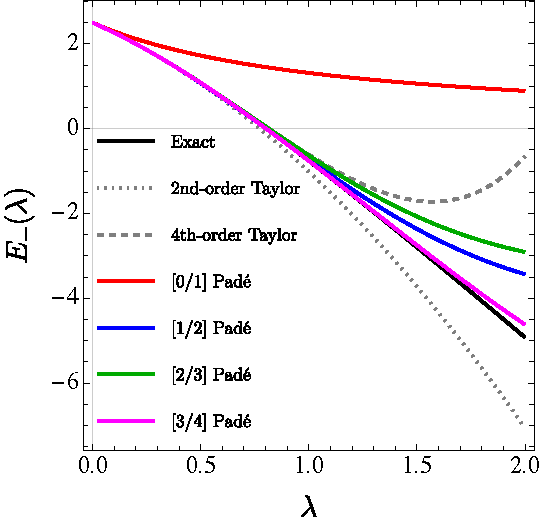
\includegraphics[width=\linewidth]{PadeRMP}
    \caption{\label{fig:PadeRMP}
    RMP ground-state energy as a function of $\lambda$ obtained using various resummation techniques at $U/t = 4.5$.}
\end{figure}
%%%%%%%%%%%%%%%%%

%==========================================%
\subsection{Quadratic approximant}
%==========================================%
In a nutshell, the idea behind quadratic approximant is to model the singularity structure of the energy function $E(\lambda)$ via a generalised version of the square-root singularity expression \cite{Mayer_1985,Goodson_2011,Goodson_2019}
\begin{equation}
	\label{eq:QuadApp}
	E(\lambda) = \frac{1}{2 Q(\lambda)} \qty[ P(\lambda) \pm \sqrt{P^2(\lambda) - 4 Q(\lambda) R(\lambda)} ]
\end{equation}
where 
\begin{align}
	\label{eq:PQR}
	P(\lambda) & = \sum_{k=0}^{d_P} p_k \lambda^k,
	&
	Q(\lambda) & = \sum_{k=0}^{d_Q} q_k \lambda^k, 
	&
	R(\lambda) & = \sum_{k=0}^{d_R} r_k \lambda^k 
\end{align}
are polynomials, such that $d_P + d_Q + d_R = n - 1$, and $n$ is the truncation order of the Taylor series of $E(\lambda)$.
Recasting Eq.~\eqref{eq:QuadApp} as a second-order expression in $E(\lambda)$, \ie,
\begin{equation}
	Q(\lambda) E^2(\lambda) - P(\lambda) E(\lambda) + R(\lambda) \sim \order*{\lambda^{n+1}}
\end{equation}
and substituting $E(\lambda$) by its $n$th-order expansion and the polynomials by their respective expressions \eqref{eq:PQR} yields $n+1$ linear equations for the coefficients $p_k$, $q_k$, and $r_k$ (where we are free to assume that $q_0 = 1$).
A quadratic approximant, characterised by the label $[d_P/d_Q,d_R]$, generates, by construction, $n_\text{bp} = \max(2d_p,d_q+d_r)$ branch points at the roots of the polynomial $P^2(\lambda) - 4 Q(\lambda) R(\lambda)$.
The diagonal sequence of quadratic approximant, \ie, $[0/0,0]$, $[1/0,0]$, $[1/0,1]$, $[1/1,1]$, $[2/1,1]$, is of particular interest.
Note that, by construction, a quadratic approximant has only two branches which hampers the faithful description of more complicated singularity structures.
As shown in Ref.~\onlinecite{Goodson_2000}, quadratic approximants provide convergent results in the most divergent cases considered by Olsen and collaborators \cite{Christiansen_1996,Olsen_1996} and Leininger \etal \cite{Leininger_2000}

For the RMP series of the Hubbard dimer, the $[0/0,0]$ and $[1/0,0]$ quadratic approximant are quite poor approximation, but its $[1/0,1]$ version already model perfectly the RMP energy function by predicting a single pair of EPs at $\lambda_\text{EP} = \pm i 4t/U$.
This is expected knowing the form of the RMP energy [see Eq.~\eqref{eq:E0MP}] which perfectly suits the purpose of quadratic approximants.

We can anticipate that the singularity structure of the UMP energy function is going to be much more challenging to model properly, and this is indeed the case as the UMP energy function contains three branches.
However, by ramping up high enough the degree of the polynomials, one is able to get an accurate estimates of the radius of convergence of the UMP series as shown in Fig.~\ref{fig:QuadUMP} and Table \ref{tab:QuadUMP}.

\titou{Here comes a discussion of Fig.~\ref{fig:QuadUMP} and Table \ref{tab:QuadUMP}.}

%%%%%%%%%%%%%%%%%
\begin{figure}
    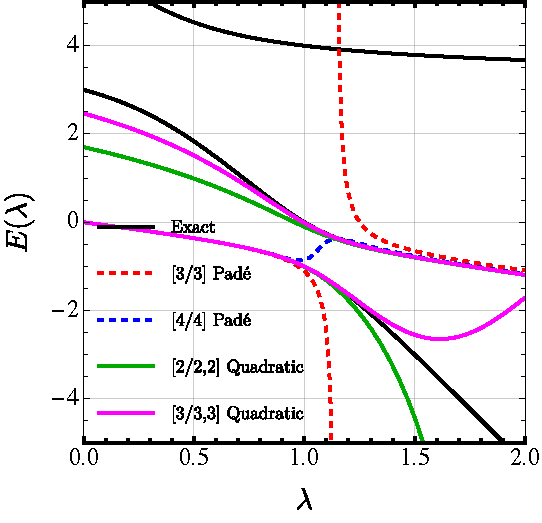
\includegraphics[width=\linewidth]{QuadUMP}
    \caption{\label{fig:QuadUMP}
    UMP energies as a function of $\lambda$ obtained using various resummation techniques at $U/t = 3$.}
\end{figure}
%%%%%%%%%%%%%%%%%

\begin{table}
	\caption{Radius of convergence $r_c$ for various resummation techniques at $U/t = 3$ and $7$.
	The truncation degree of the Taylor expansion $n$ of $E(\lambda)$ and the number of branch points $n_\text{bp} = \max(2d_p,d_q+d_r)$ generated by the quadratic approximant are also reported.
	\label{tab:QuadUMP}}
	\begin{ruledtabular}
		\begin{tabular}{llcccc}
						&			&			&					&	\mc{2}{c}{$r_c$}			\\
																		\cline{5-6}
			\mc{2}{c}{Method}		&	$n$		&	$n_\text{bp}$	&	$U/t = 3$	&	$U/t = 7$	\\
			\hline
			Pad\'e		&	[2/2]	&	4	&		&	0.97448		&	1.00030	\\
						&	[3/3]	&	6	&		&	1.14138		&	1.00448	\\
			Quadratic	&	[2/1,2]	&	6	&	4	&	1.08640		&	1.00310	\\
						&	[2/2,2]	&	7	&	4	&	1.08193		&	1.00310	\\
						&	[3/2,2]	&	8	&	6	&	1.08247		&	1.00106	\\
						&	[3/2,3]	&	9	&	6	&	1.07069		&	1.00239	\\
						&	[3/3,3]	&	10	&	6	&	1.07064		&	1.00239	\\
			Exact		&			&		&		&	1.06917		&	1.00239\\
		\end{tabular}
	\end{ruledtabular}
\end{table}

%==========================================%
\subsection{Analytic continuation}
%==========================================%

Recently, Mih\'alka \textit{et al.} studied the partitioning effect on the convergence properties of Rayleigh-Schr\"odinger perturbation theory by considering the MP and the EN partitioning as well as an alternative partitioning \cite{Mihalka_2017a} (see also Ref.~\onlinecite{Surjan_2000}).
Taking as an example (in particular) the water molecule at equilibrium and at stretched geometries, they could estimate the radius of convergence via a quadratic Pad\'e approximant and convert divergent perturbation expansions to convergent ones in some cases thanks to a judicious choice of the level shift parameter.
In a subsequent study by the same group, \cite{Mihalka_2017b} they use analytic continuation techniques to resum divergent MP series \cite{Goodson_2011} taking again as an example the water molecule in a stretched geometry.
In a nutshell, their idea consists in calculating the energy of the system for several values of $\lambda$ for which the MP series is rapidly convergent (\ie, for $\lambda < r_c$), and to extrapolate the final energy to the physical system at $\lambda = 1$ via a polynomial- or Pad\'e-based fit. 
However, the choice of the functional form of the fit remains a subtle task.
This technique was first generalised by using complex scaling parameters and applying analytic continuation by solving the Laplace equation, \cite{Surjan_2018} and then further improved thanks to Cauchy's integral formula \cite{Mihalka_2019}
\begin{equation}
	\label{eq:Cauchy}
	\frac{1}{2\pi i} \oint_{\gamma} \frac{E(\lambda)}{\lambda - a} = E(a),
\end{equation}
which states that the value of the energy can be computed at $\lambda=a$ inside the complex contour $\gamma$ only by the knowledge of its values on the same contour.
Their method consists in refining self-consistently the values of $E(\lambda)$ computed on a contour going through the physical point at $\lambda = 1$ and encloses points of the ``trusted'' region (where the MP series is convergent). The shape of this contour is arbitrary but no singularities are allowed inside the contour to ensure $E(\lambda)$ is analytic. 
When the values of $E(\lambda)$ on the so-called contour are converged, Cauchy's integrals formula \eqref{eq:Cauchy} is invoked to compute the values at $E(\lambda=1)$ which corresponds to the final estimate of the FCI energy.
The authors illustrate this protocol on the dissociation curve of \ce{LiH} and the stretched water molecule showing encouraging results. \cite{Mihalka_2019} 

%%%%%%%%%%%%%%%%%%%%
\section{Conclusion}
%%%%%%%%%%%%%%%%%%%%

In order to model accurately chemical systems, one must choose, in a ever growing zoo of methods, which computational protocol is adapted to the system of interest.
This choice can be, moreover, motivated by the type of properties that one is interested in.
That means that one must understand the strengths and weaknesses of each method, \ie, why one method might fail in some cases and work beautifully in others. 
We have seen that for methods relying on perturbation theory, their successes and failures are directly connected to the position of EPs in the complex plane. 
Exhaustive studies have been performed on the causes of failure of MP perturbation theory. 
First, it was understood that, for chemical systems for which the HF Slater determinant is a poor approximation to the exact wave function, MP perturbation theory fails too. 
Such systems can be, for example, molecules where the exact ground-state wave function is dominated by more than one configuration, \ie, multi-reference systems. 
More preoccupying cases were also reported. 
For instance, it has been shown that systems considered as well understood (\eg, \ce{Ne}) can exhibit divergent behaviour when the basis set is augmented with diffuse functions. 
Later, these erratic behaviours of the perturbation series were investigated and rationalised in terms of avoided crossings and singularities in the complex plane. 
It was shown that the singularities can be classified in two families. 
The first family includes $\alpha$ singularities resulting from a large avoided crossing between the ground state and a low-lying doubly-excited states. 
The $\beta$ singularities, which constitutes the second family, are artefacts generated by the incompleteness of the Hilbert space, and they are directly connected to an ionisation phenomenon occurring in the complete Hilbert space. 
These singularities are close to the real axis and connected with sharp avoided crossing between the ground state and a highly diffuse state. 
We have found that the $\beta$ singularities modelling the ionisation phenomenon described by Sergeev and Goodson are actually part of a more general class of singularities. 
Indeed, those singularities close to the real axis are connected to quantum phase transitions and symmetry breaking, and theoretical physics have demonstrated that the behaviour of the EPs depends of the type of transitions from which the EPs result (first or higher orders, ground state or excited state transitions).
To conclude, this work shows that our understanding of the singularity structure of the energy is still incomplete but we hope that it opens new perspectives for the understanding of the physics of EPs in electronic structure theory.

%%%%%%%%%%%%%%%%%%%%%%%%
\begin{acknowledgements}
%%%%%%%%%%%%%%%%%%%%%%%%
This project has received funding from the European Research Council (ERC) under the European Union's Horizon 2020 research and innovation programme (Grant agreement No.~863481).
HGAB gratefully acknowledges New College, Oxford for funding through the Astor Junior Research Fellowship.
%%%%%%%%%%%%%%%%%%%%%%
\end{acknowledgements}
%%%%%%%%%%%%%%%%%%%%%%

%%%%%%%%%%%%%%%%%%%%%%
\bibliography{EPAWTFT}
%%%%%%%%%%%%%%%%%%%%%%

\end{document}
